The formulae for insolation calculations are taken from \citemarsenv{Appelbaum1989}, \citemarsenv{Appelbaum1990}, \citemarsenv{Appelbaum1991}, and \citemarsenv{Appelbaum1993}. For the purpose of this thesis, the formulae are implemented into an R package to be used in mission analysis power budgets and energy predictions. Both \citemarsenv{Appelbaum1990} and \citemarsenv{Appelbaum1993} include tables listing pre-calculated insolation values for horizontal and inclined surfacesnat \ac{VL1} and \ac{VL2} locations. These published values are used to validate the R implementation of the insolation formulae. This chapter compares the published and calculated insolation values with each other in order to verify and validate the developed R package.


\section{Horizontal Surface}
\subsection{At Viking Lander 1 (VL1)}
\refFig{fig:sub:comparative-global-insolation-at-vl1-horizontal-daily-variations} shows that calculated values are consistently lower than those published in \citemarsenv{Appelbaum1990}. Both daily variations closely follow the same pattern. \refFig{fig:sub:comparative-global-insolation-at-vl1-horizontal-percentage-differences} reveals that the differences between calculated and published values range between \SI{2.8}{\percent} and \SI{3.3}{\percent}. Differences larger than \SI{3}{\percent} are restricted to $\tau$ values between 0.5 and 1.9.

\begin{figure}[h]
\captionsetup[subfigure]{justification=centering}
\vspace{-2ex}
\centering
    %% setup sizes
    \setlength{\subfigureWidth}{0.50\textwidth}
    \setlength{\graphicsHeight}{60mm}
    %% kill hyper-link highlighting
    \hypersetup{hidelinks=true}%
    %% the figures
    \begin{subfigure}[t]{\subfigureWidth}
        \centering
            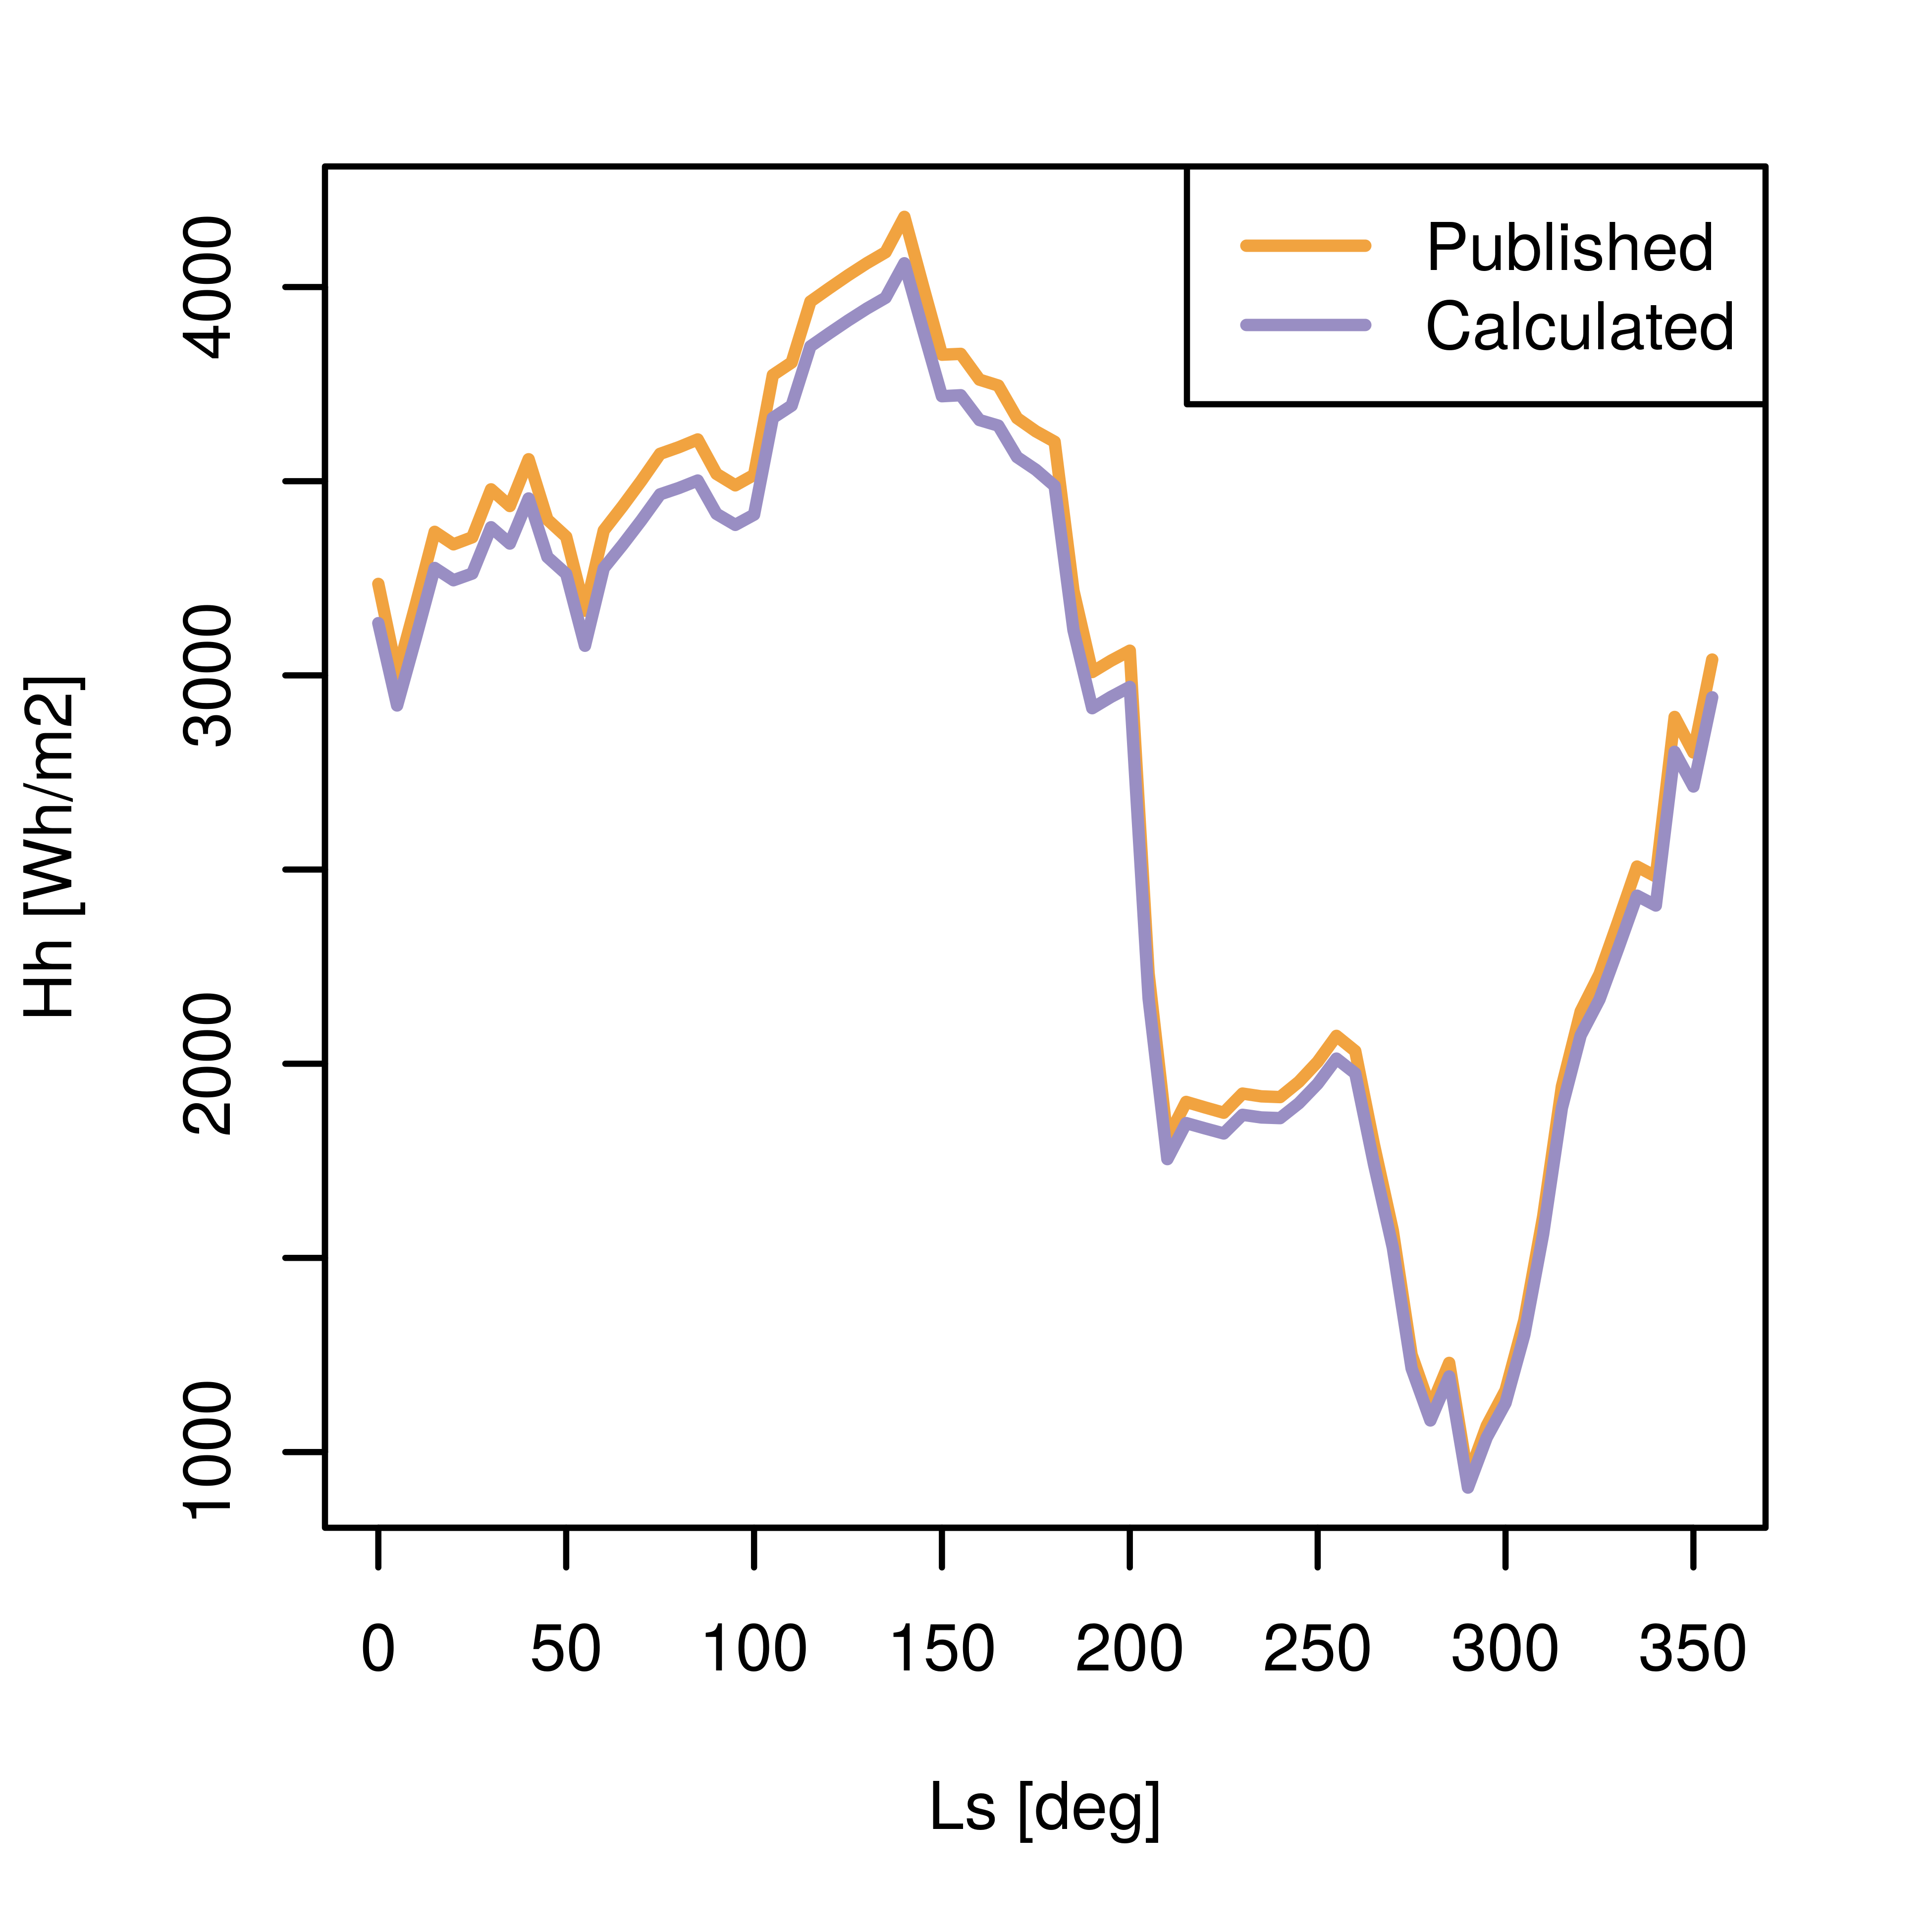
\includegraphics[height=\graphicsHeight]{sections/appendix/insolation-calculation-verification/plots/hh-exp-calc-at-vl1.png}
            \subcaption{Daily variations}
            \label{fig:sub:comparative-global-insolation-at-vl1-horizontal-daily-variations}
    \end{subfigure}\hfill
    \begin{subfigure}[t]{\subfigureWidth}
        \centering
            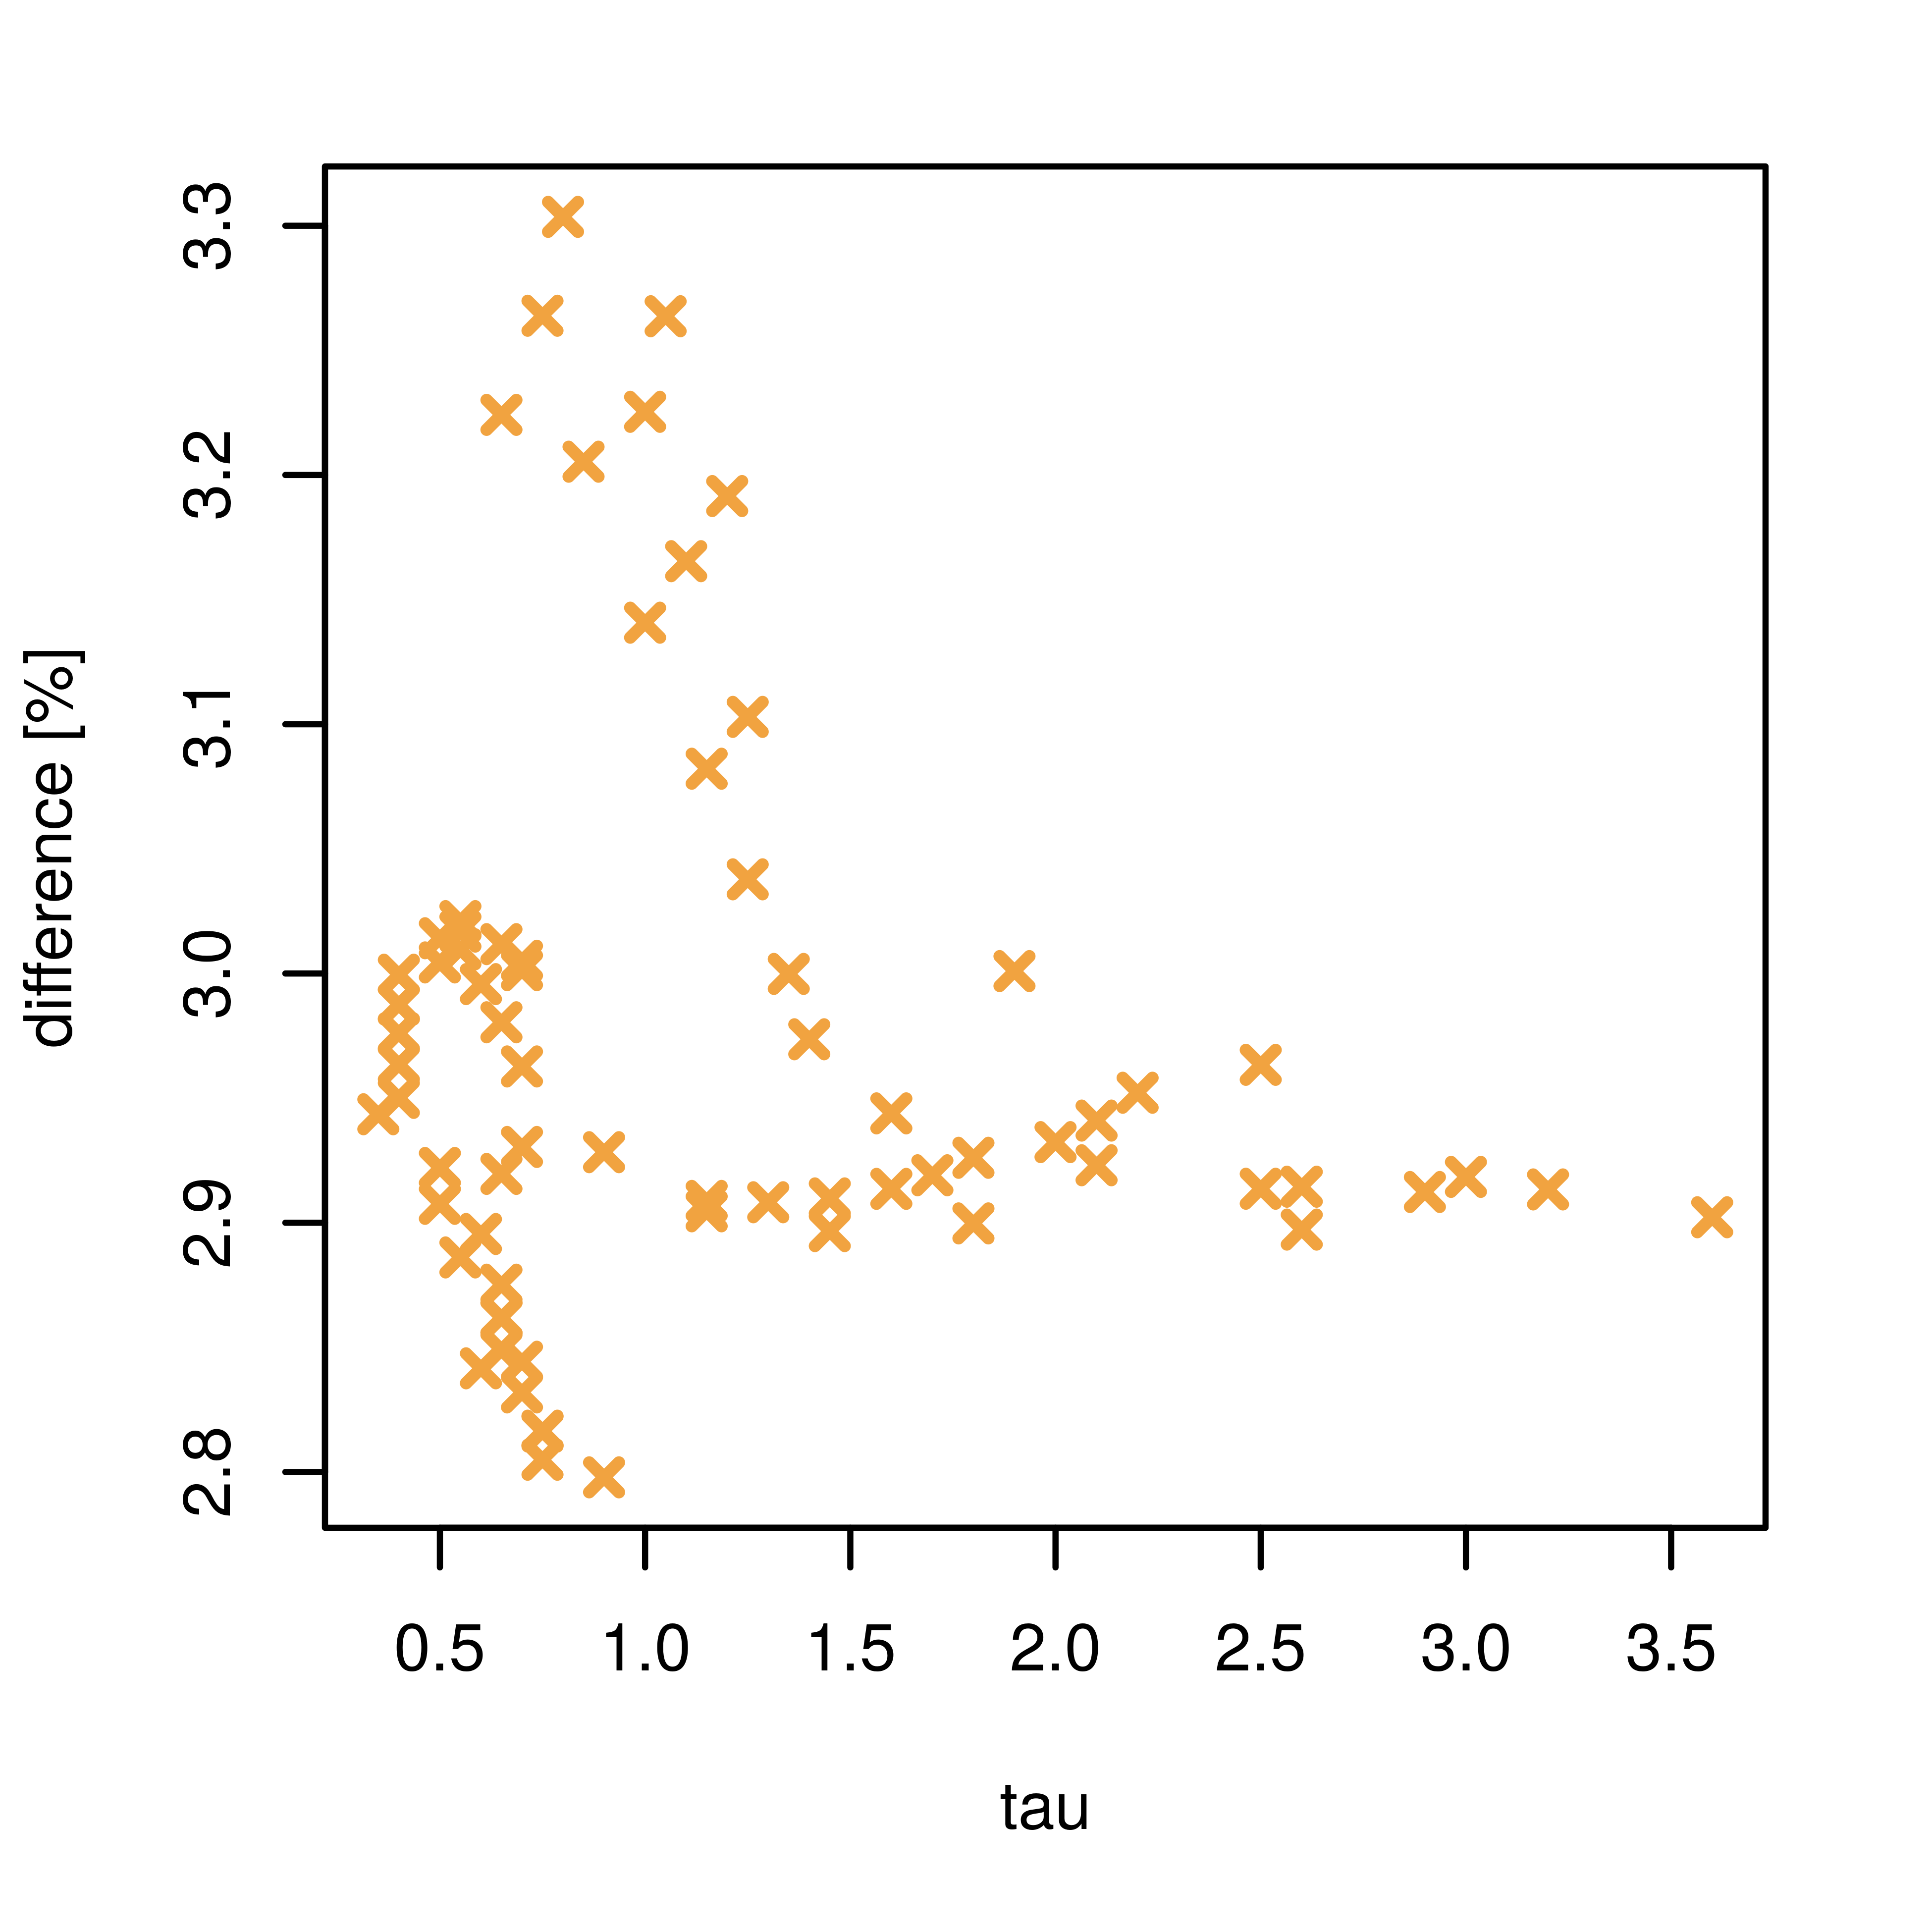
\includegraphics[height=\graphicsHeight]{sections/appendix/insolation-calculation-verification/plots/hh-diff-bet-exp-calc-at-vl1.png}
            \subcaption{Differences as a function of optical depth}
            \label{fig:sub:comparative-global-insolation-at-vl1-horizontal-percentage-differences}
    \end{subfigure}\\[0.8ex]
    \caption[Daily global insolations at Viking Lander 1 on a horizontal surface]
    {Daily global insolations at \ac{VL1} on a horizontal surface.}
    \label{fig:plot:comparative-global-insolation-at-vl1-horizontal}
\vspace{-2ex}
\end{figure}

\subsection{At Viking Lander 2 (VL2)}
\refFig{fig:sub:comparative-global-insolation-at-vl2-horizontal-daily-variations} shows that calculated values are consistently lower than those published in \citemarsenv{Appelbaum1990}. Both daily variations closely follow the same patterns. \refFig{fig:sub:comparative-global-insolation-at-vl2-horizontal-percentage-differences} reveals that the differences between calculated and published values range between \SI{2.3}{\percent} and \SI{3.9}{\percent}. Differences larger than \SI{3}{\percent} are more frequent for large $\tau$ values, particularly above 1.

\begin{figure}[h]
\captionsetup[subfigure]{justification=centering}
%\vspace{-2ex}
\centering
    %% setup sizes
    \setlength{\subfigureWidth}{0.50\textwidth}
    \setlength{\graphicsHeight}{60mm}
    %% kill hyper-link highlighting
    \hypersetup{hidelinks=true}%
    %% the figures
    \begin{subfigure}[t]{\subfigureWidth}
        \centering
            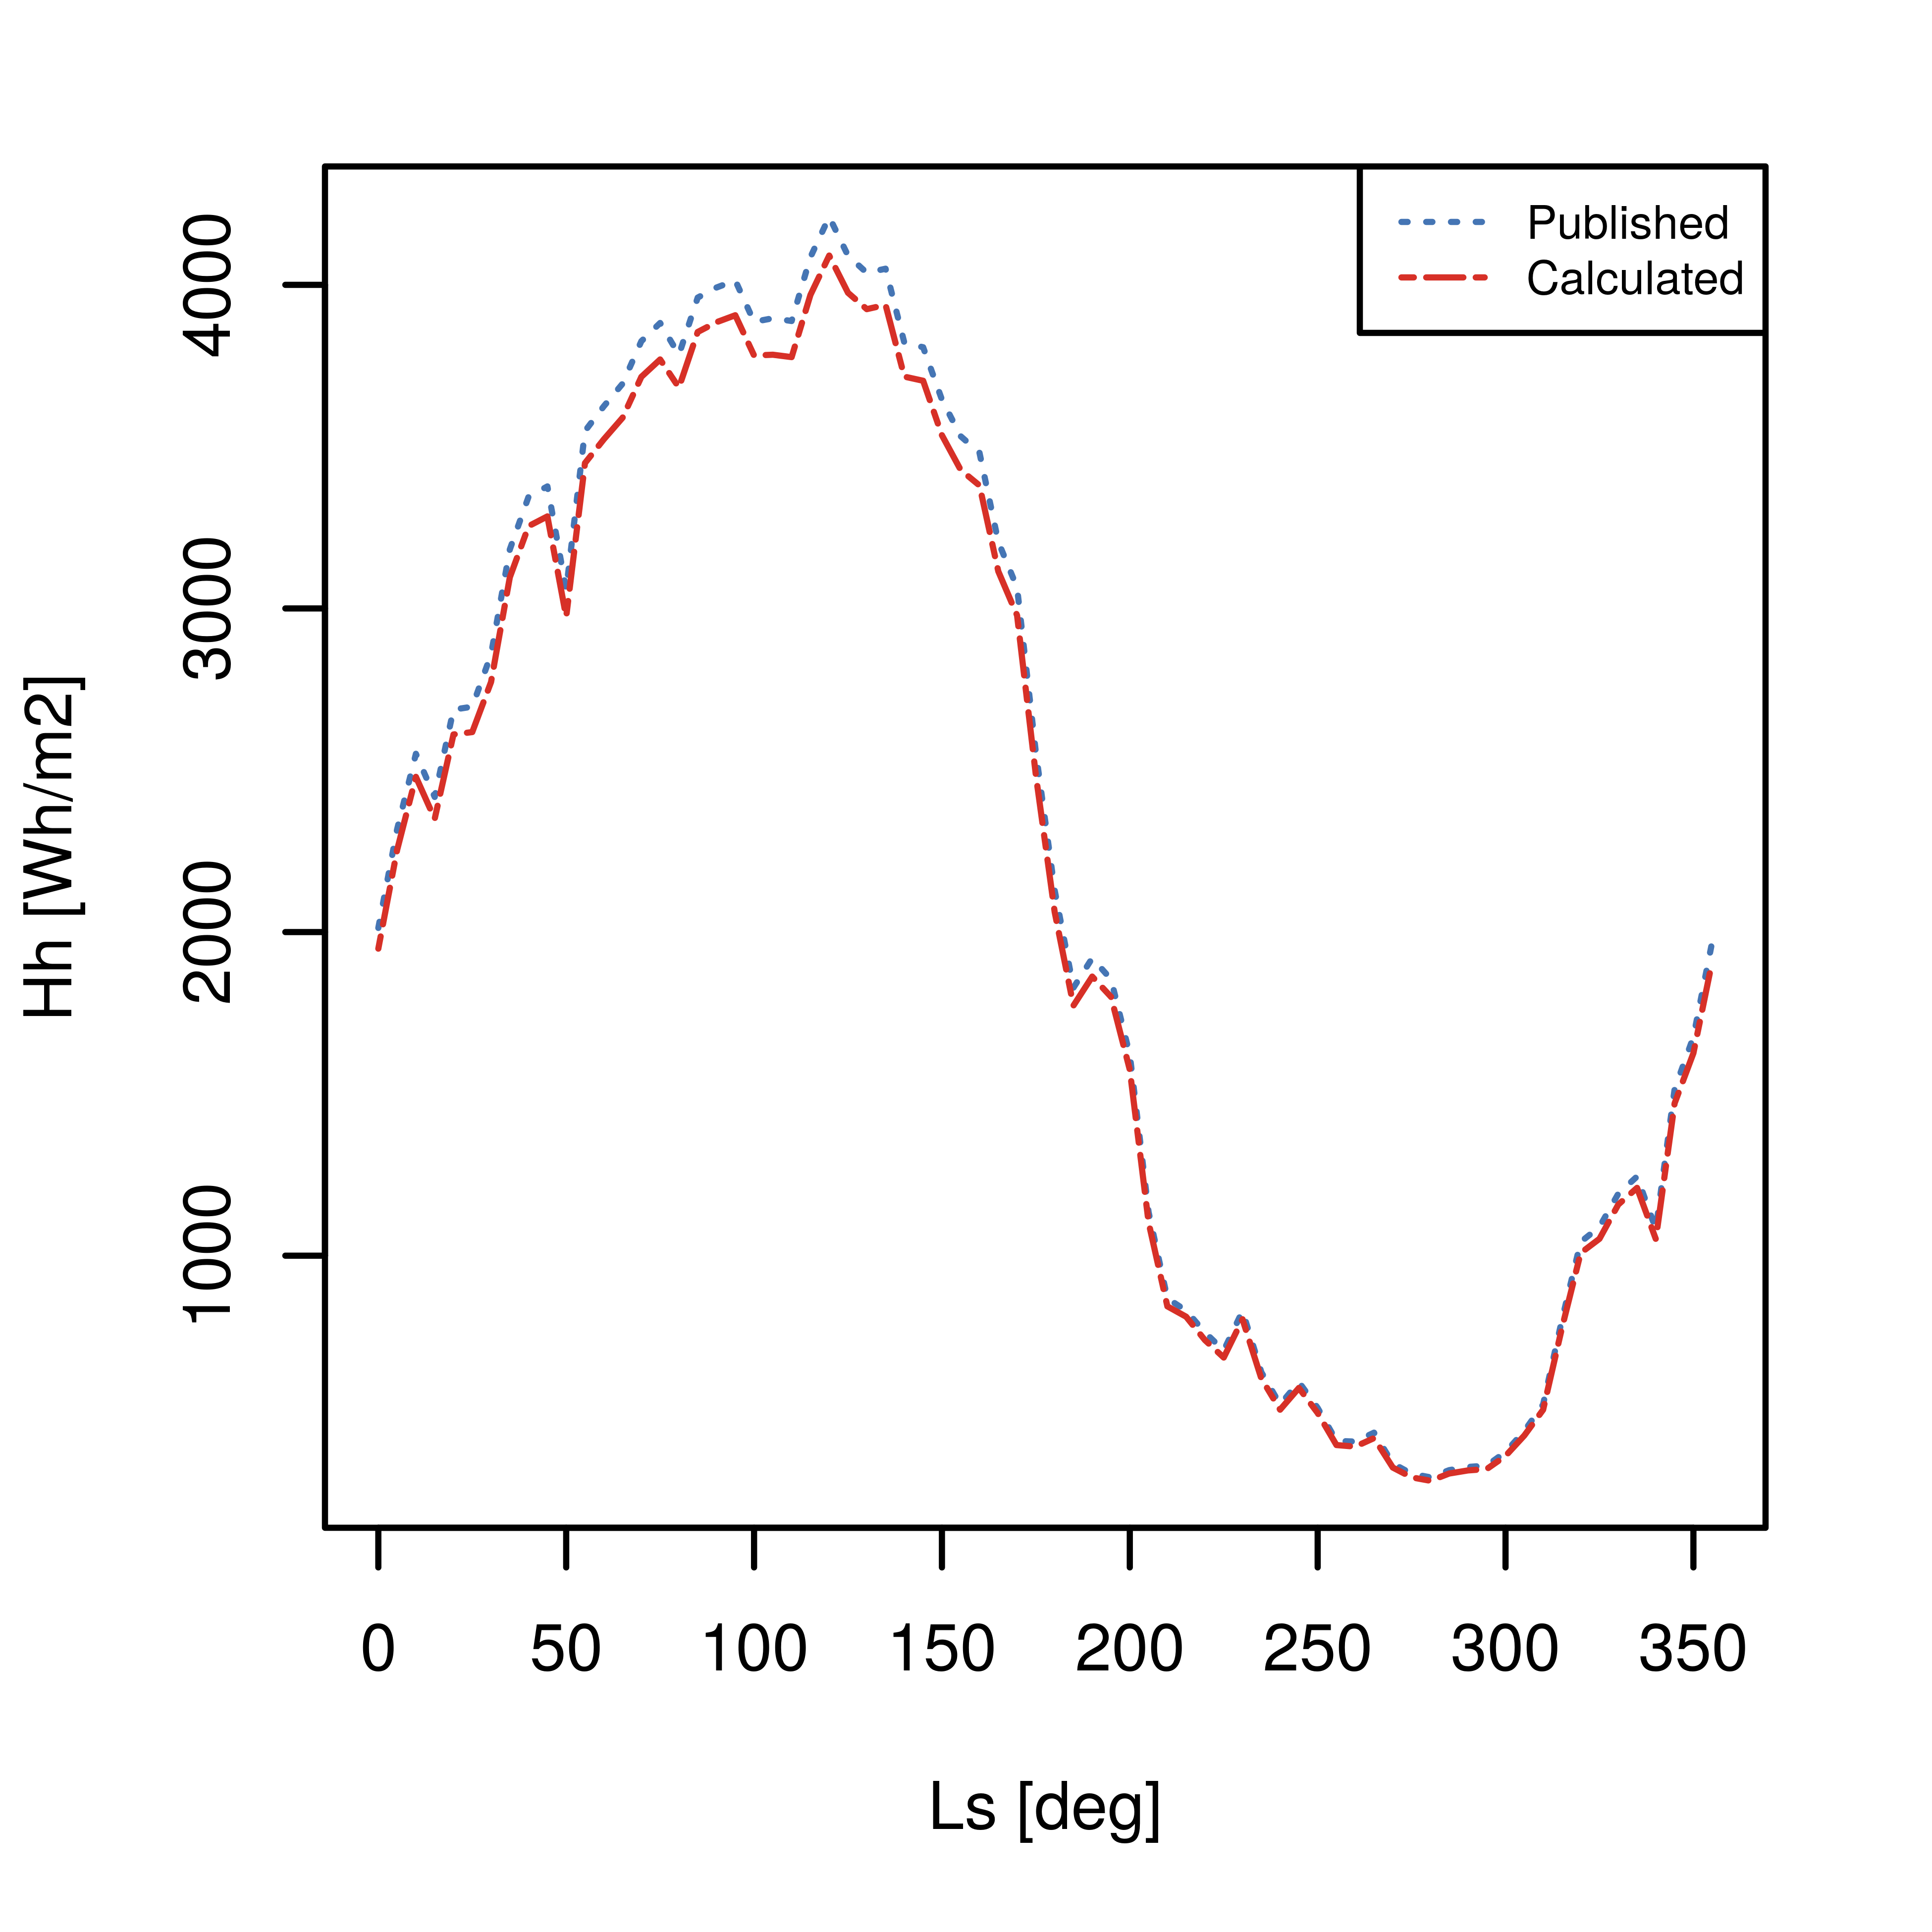
\includegraphics[height=\graphicsHeight]{sections/appendix/insolation-calculation-verification/plots/hh-exp-calc-at-vl2.png}
            \subcaption{Daily variations}
            \label{fig:sub:comparative-global-insolation-at-vl2-horizontal-daily-variations}
    \end{subfigure}\hfill
    \begin{subfigure}[t]{\subfigureWidth}
        \centering
            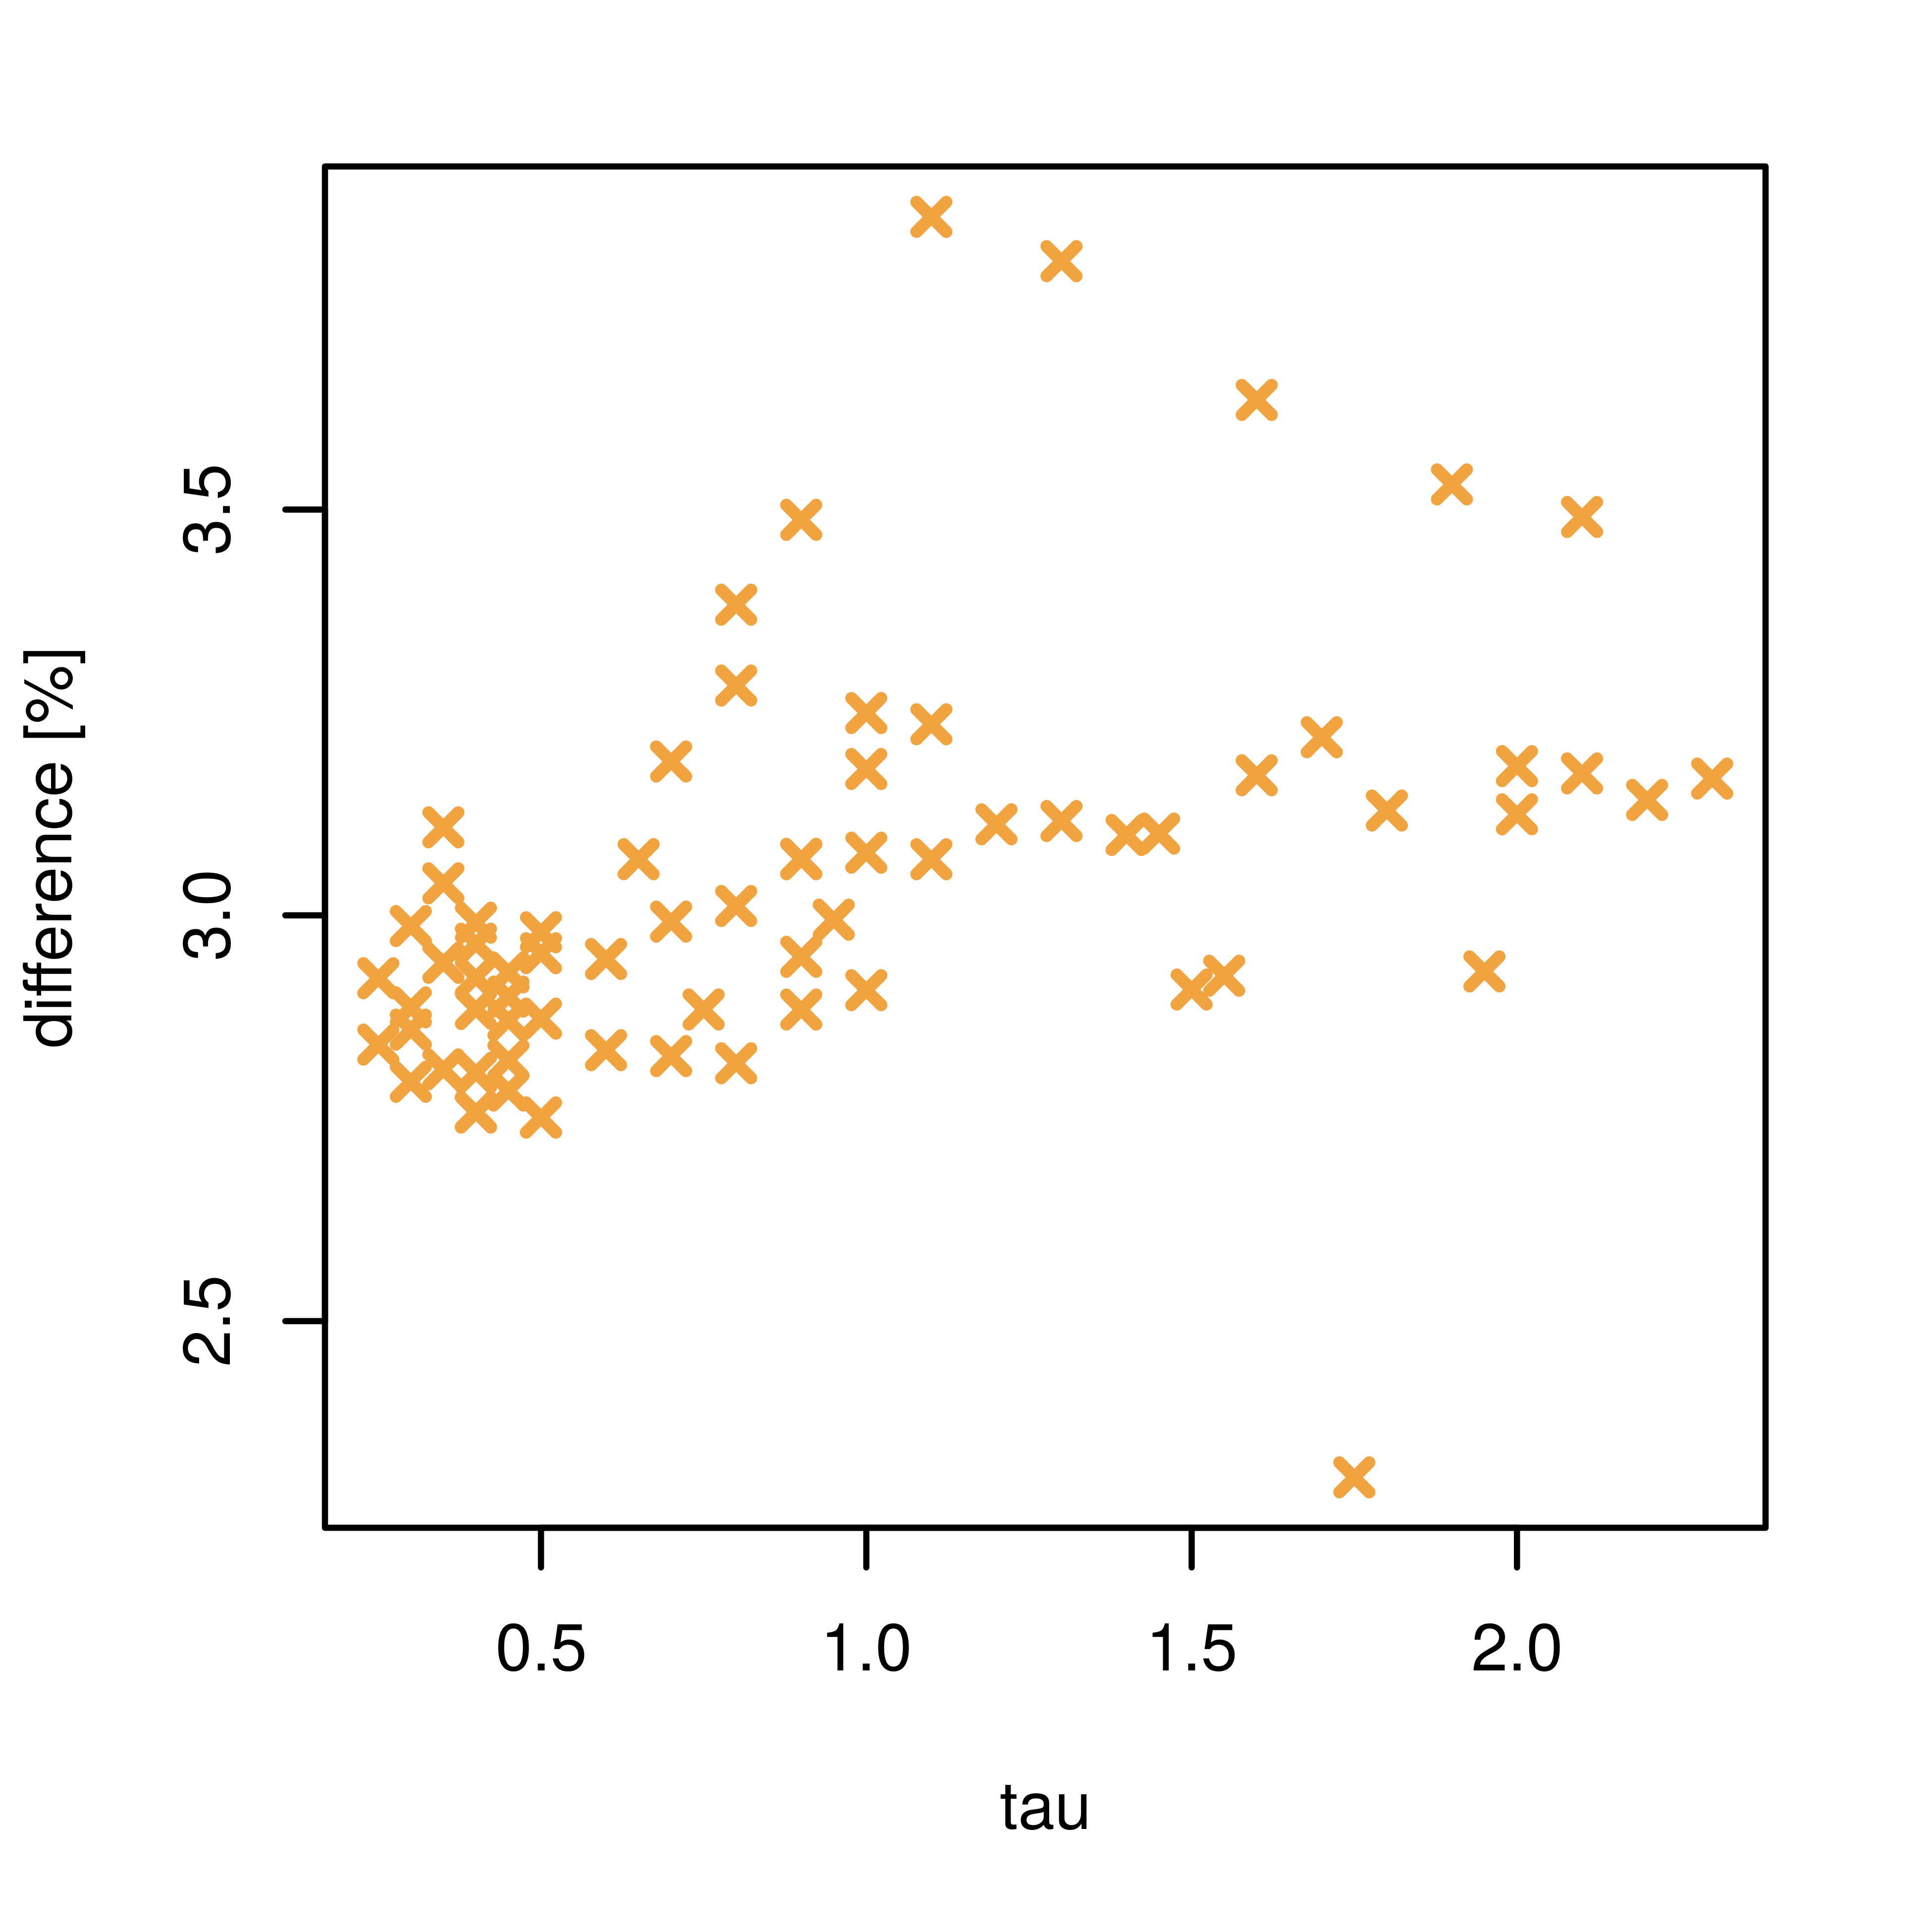
\includegraphics[height=\graphicsHeight]{sections/appendix/insolation-calculation-verification/plots/hh-diff-bet-exp-calc-at-vl2.png}
            \subcaption{Differences as a function of optical depth}
            \label{fig:sub:comparative-global-insolation-at-vl2-horizontal-percentage-differences}
    \end{subfigure}\\[0.8ex]
    \caption[Daily global insolations at Viking Lander 2 on a horizontal surface]
    {Daily global insolations at \ac{VL2} on a horizontal surface.}
    \label{fig:plot:comparative-global-insolation-at-vl2-horizontal}
\vspace{-2ex}
\end{figure}

\section{Inclined Surface with Beta Equals Phi}
\subsection{At Viking Lander 1 (VL1)}
\refFig{fig:sub:comparative-global-insolation-at-vl1-beta-equals-phi-daily-variations} shows that calculated values are consistently lower than those published in \citemarsenv{Appelbaum1993}. Both daily variations closely follow the same pattern. \refFig{fig:sub:comparative-global-insolation-at-vl1-beta-equals-phi-percentage-differences} reveals that the differences between calculated and published values range between \SI{2.1}{\percent} and \SI{3.1}{\percent}. Differences larger than \SI{2.5}{\percent} are more frequent for small $\tau$ values, particularly below 1.

\begin{figure}[h]
\captionsetup[subfigure]{justification=centering}
\vspace{-2ex}
\centering
    %% setup sizes
    \setlength{\subfigureWidth}{0.50\textwidth}
    \setlength{\graphicsHeight}{60mm}
    %% kill hyper-link highlighting
    \hypersetup{hidelinks=true}%
    %% the figures
    \begin{subfigure}[t]{\subfigureWidth}
        \centering
            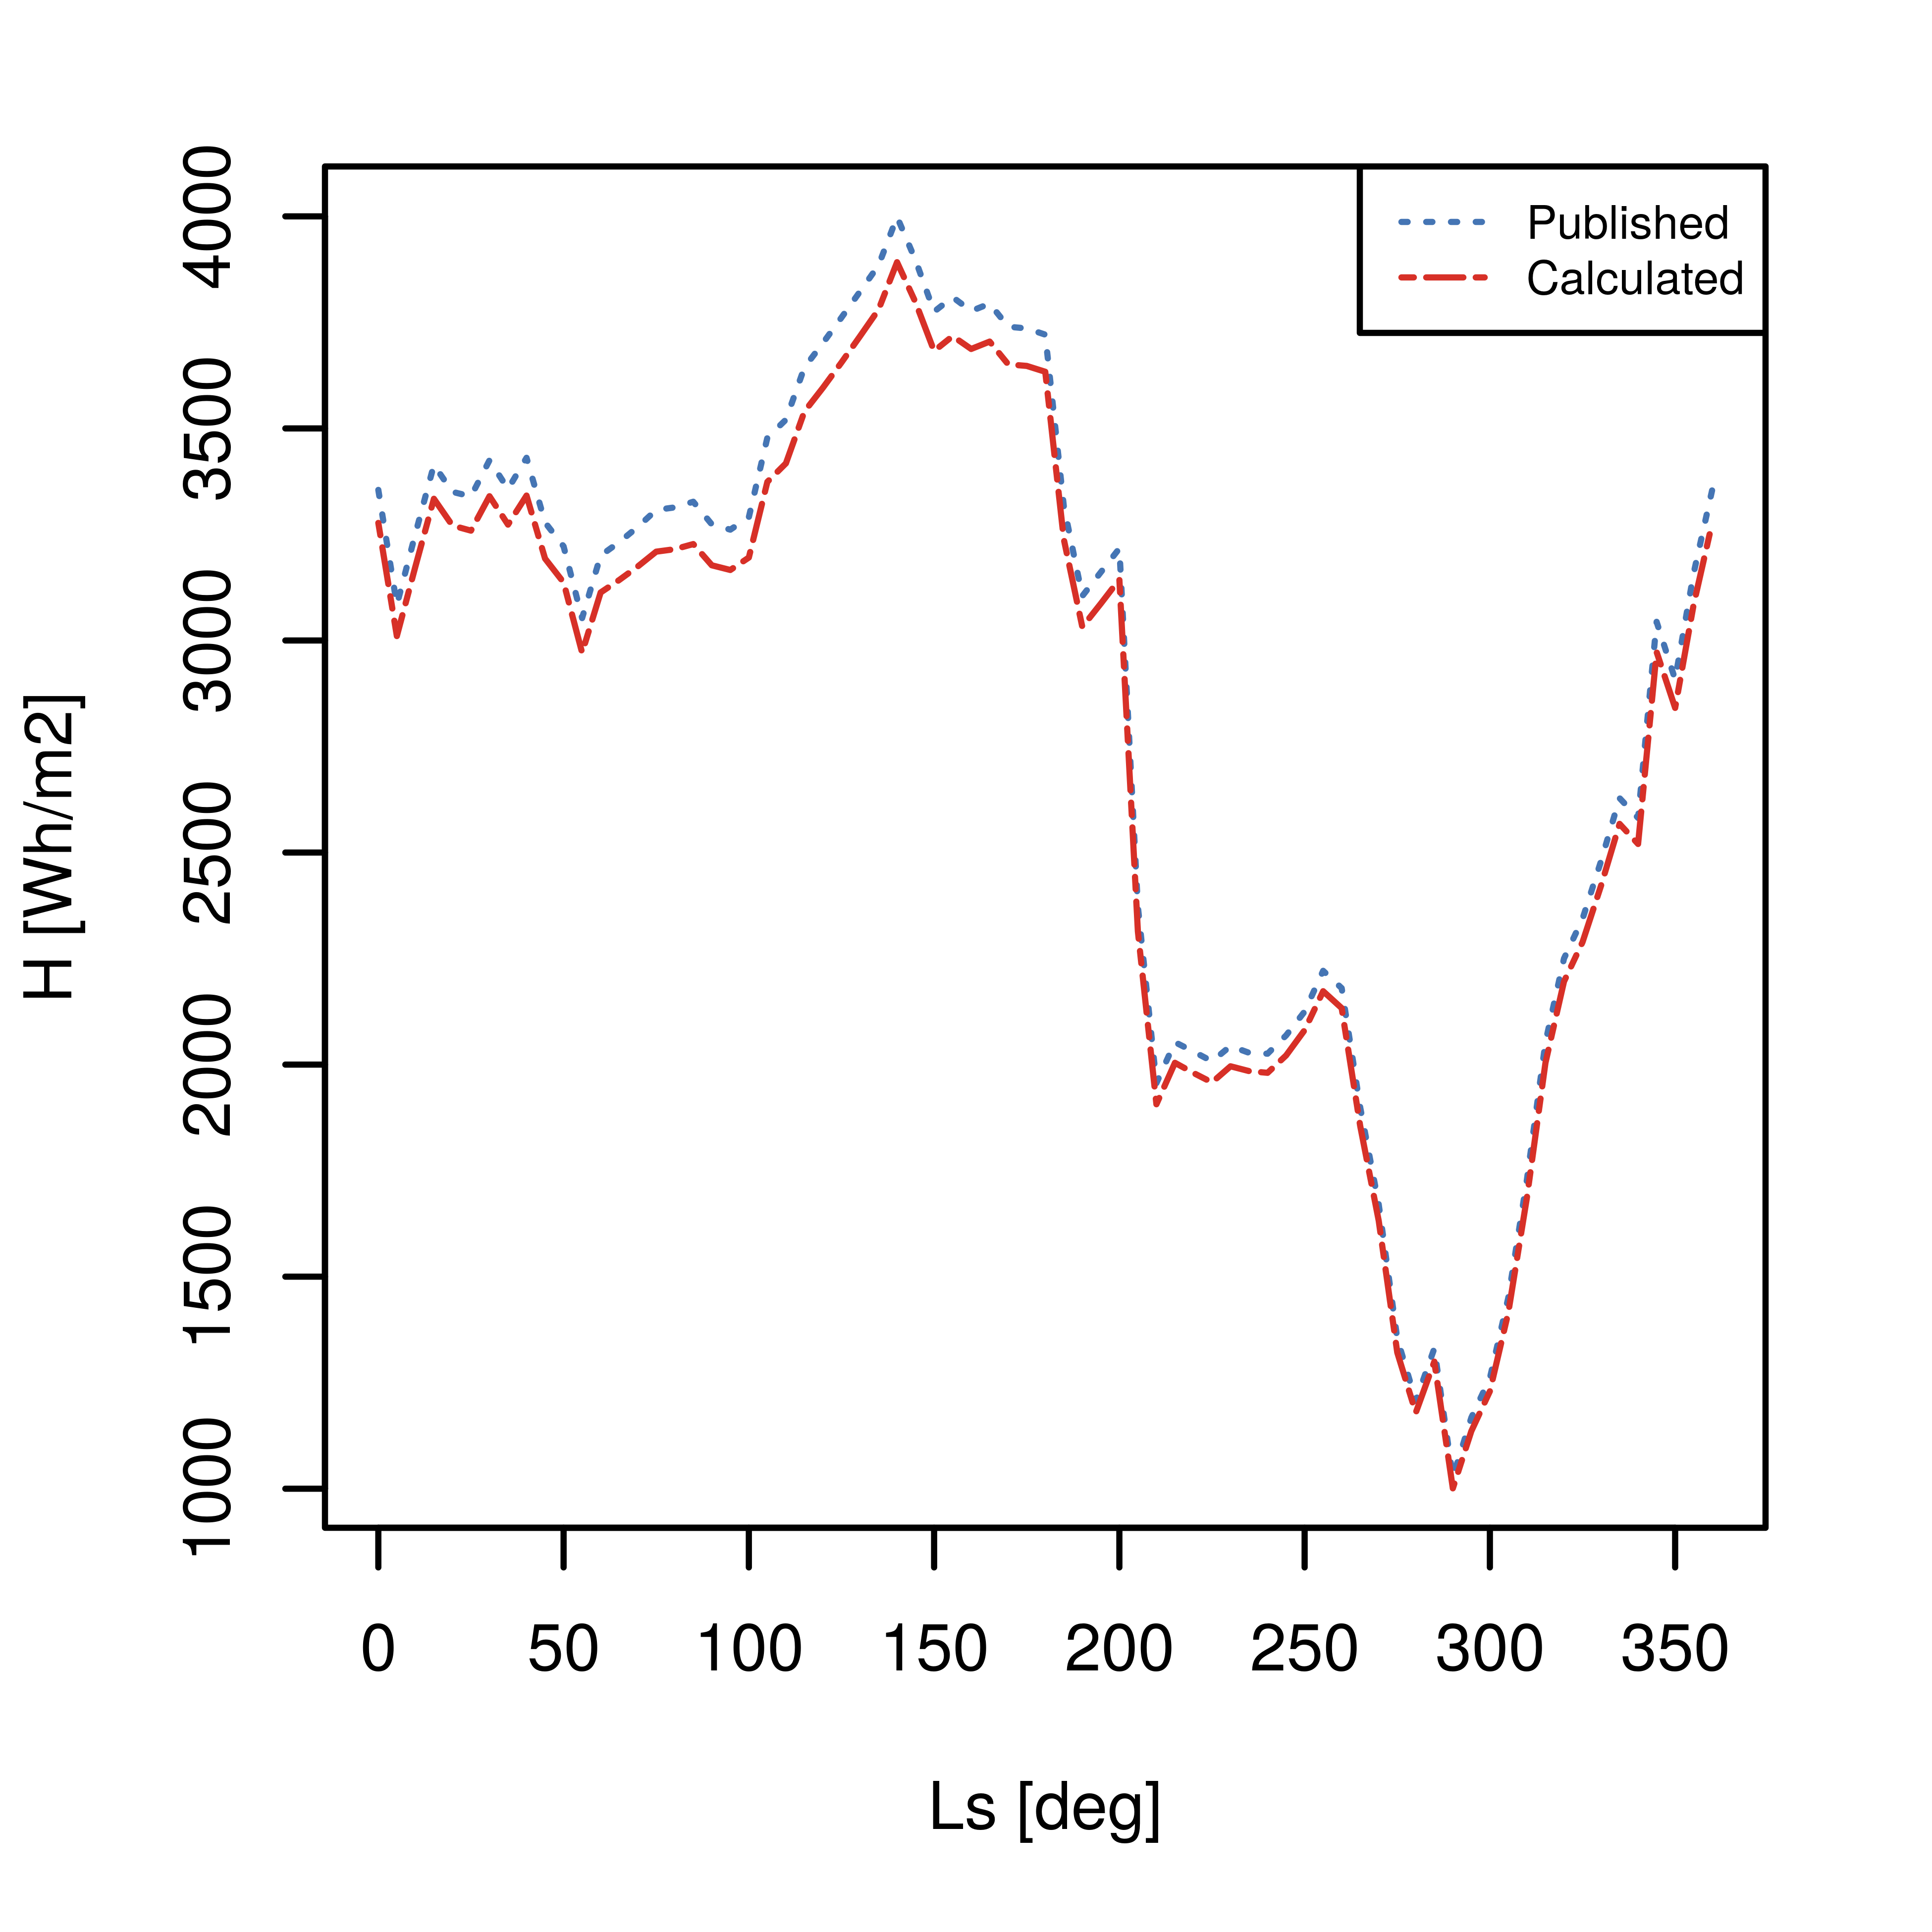
\includegraphics[height=\graphicsHeight]{sections/appendix/insolation-calculation-verification/plots/h-exp-calc-at-vl1-with-beta-223-deg.png}
            \subcaption{Daily variations}
            \label{fig:sub:comparative-global-insolation-at-vl1-beta-equals-phi-daily-variations}
    \end{subfigure}\hfill
    \begin{subfigure}[t]{\subfigureWidth}
        \centering
            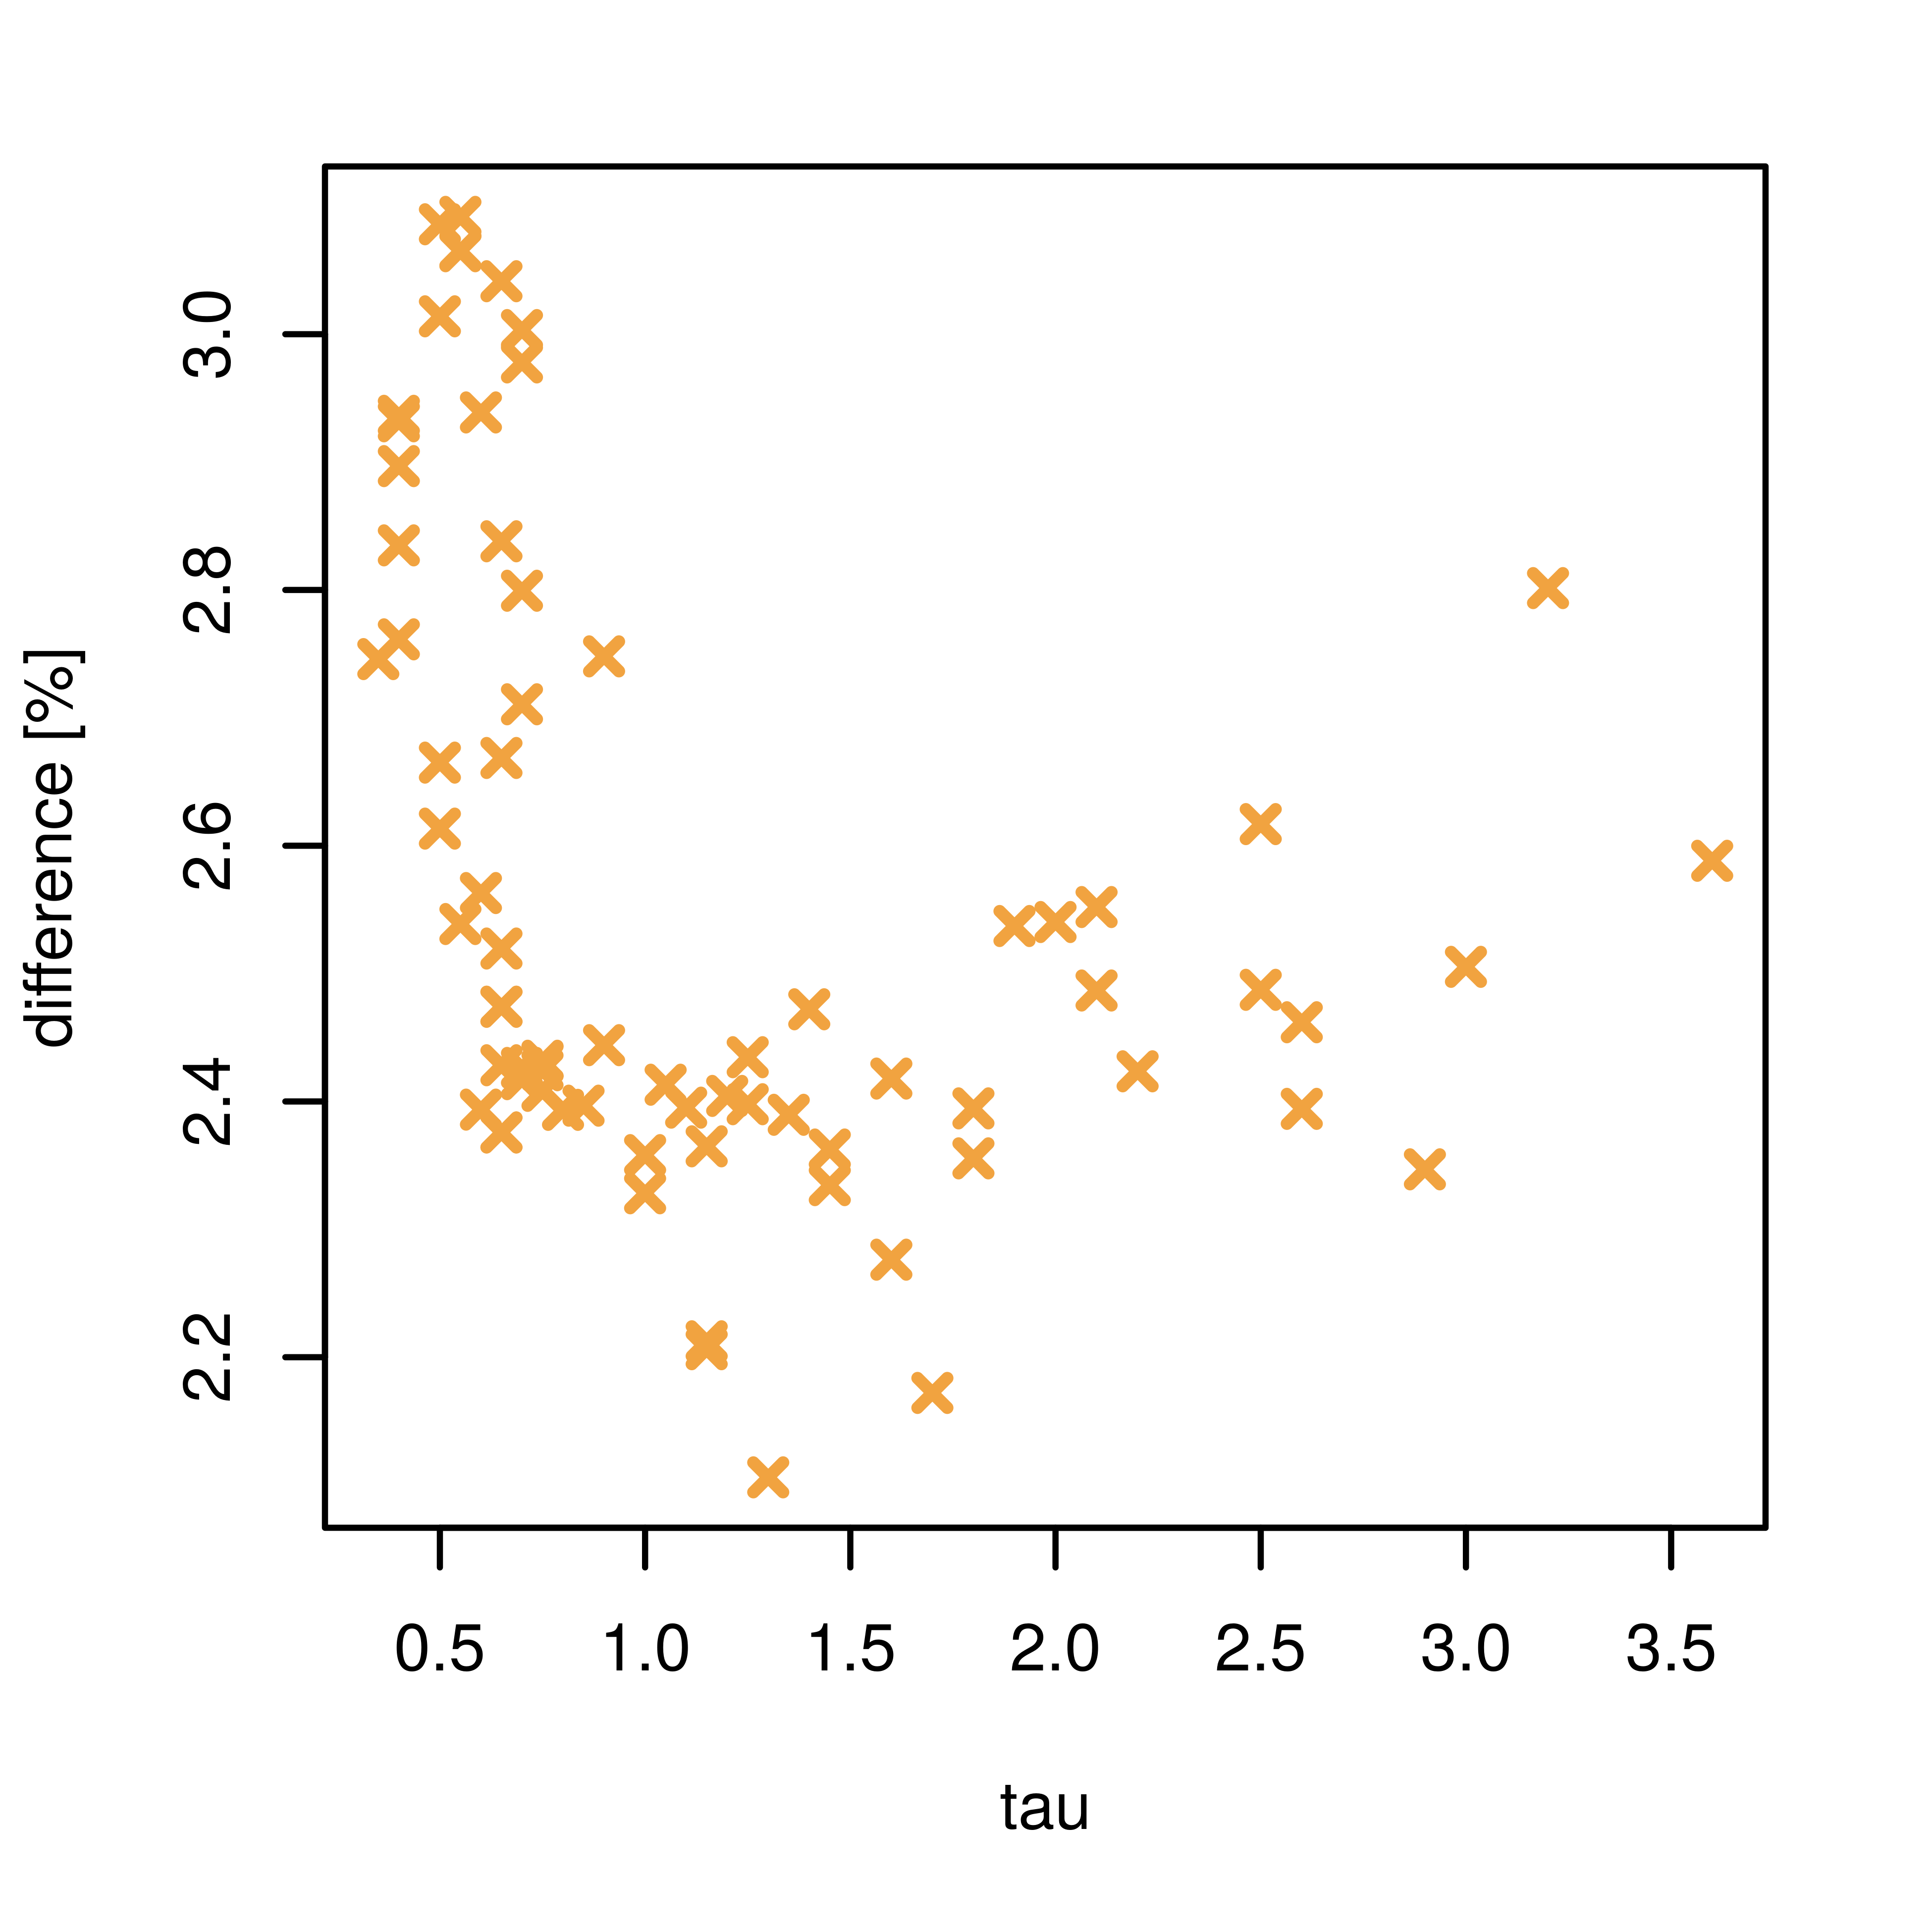
\includegraphics[height=\graphicsHeight]{sections/appendix/insolation-calculation-verification/plots/h-diff-bet-exp-calc-at-vl1-with-beta-223-deg.png}
            \subcaption{Differences as a function of optical depth}
            \label{fig:sub:comparative-global-insolation-at-vl1-beta-equals-phi-percentage-differences}
    \end{subfigure}\\[0.8ex]
    \caption[Daily global insolations at Viking Lander 1 on an inclined surface with $\beta=\SI{22.3}{\degree}$]
    {Daily global insolations at \ac{VL1} on an inclined surface with $\beta=\SI{22.3}{\degree}$.}
    \label{fig:plot:comparative-global-insolation-at-vl1-beta-equals-phi}
\vspace{-2ex}
\end{figure}

\subsection{At Viking Lander 2 (VL2)}
\refFig{fig:sub:comparative-global-insolation-at-vl2-beta-equals-phi-daily-variations} shows that calculated values are consistently lower than those published in \citemarsenv{Appelbaum1993}. Both daily variations closely follow the same patterns. \refFig{fig:sub:comparative-global-insolation-at-vl2-beta-equals-phi-percentage-differences} reveals that the differences between calculated and published values range between \SI{0.4}{\percent} and \SI{6.6}{\percent}. Differences larger than \SI{3}{\percent} are more frequent for small $\tau$ values, particularly from 0.25 to 0.5 with differences larger than \SI{6}{\percent} for $\tau$ 0.4 and 0.5.

\begin{figure}[h]
\captionsetup[subfigure]{justification=centering}
%\vspace{-2ex}
\centering
    %% setup sizes
    \setlength{\subfigureWidth}{0.50\textwidth}
    \setlength{\graphicsHeight}{60mm}
    %% kill hyper-link highlighting
    \hypersetup{hidelinks=true}%
    %% the figures
    \begin{subfigure}[t]{\subfigureWidth}
        \centering
            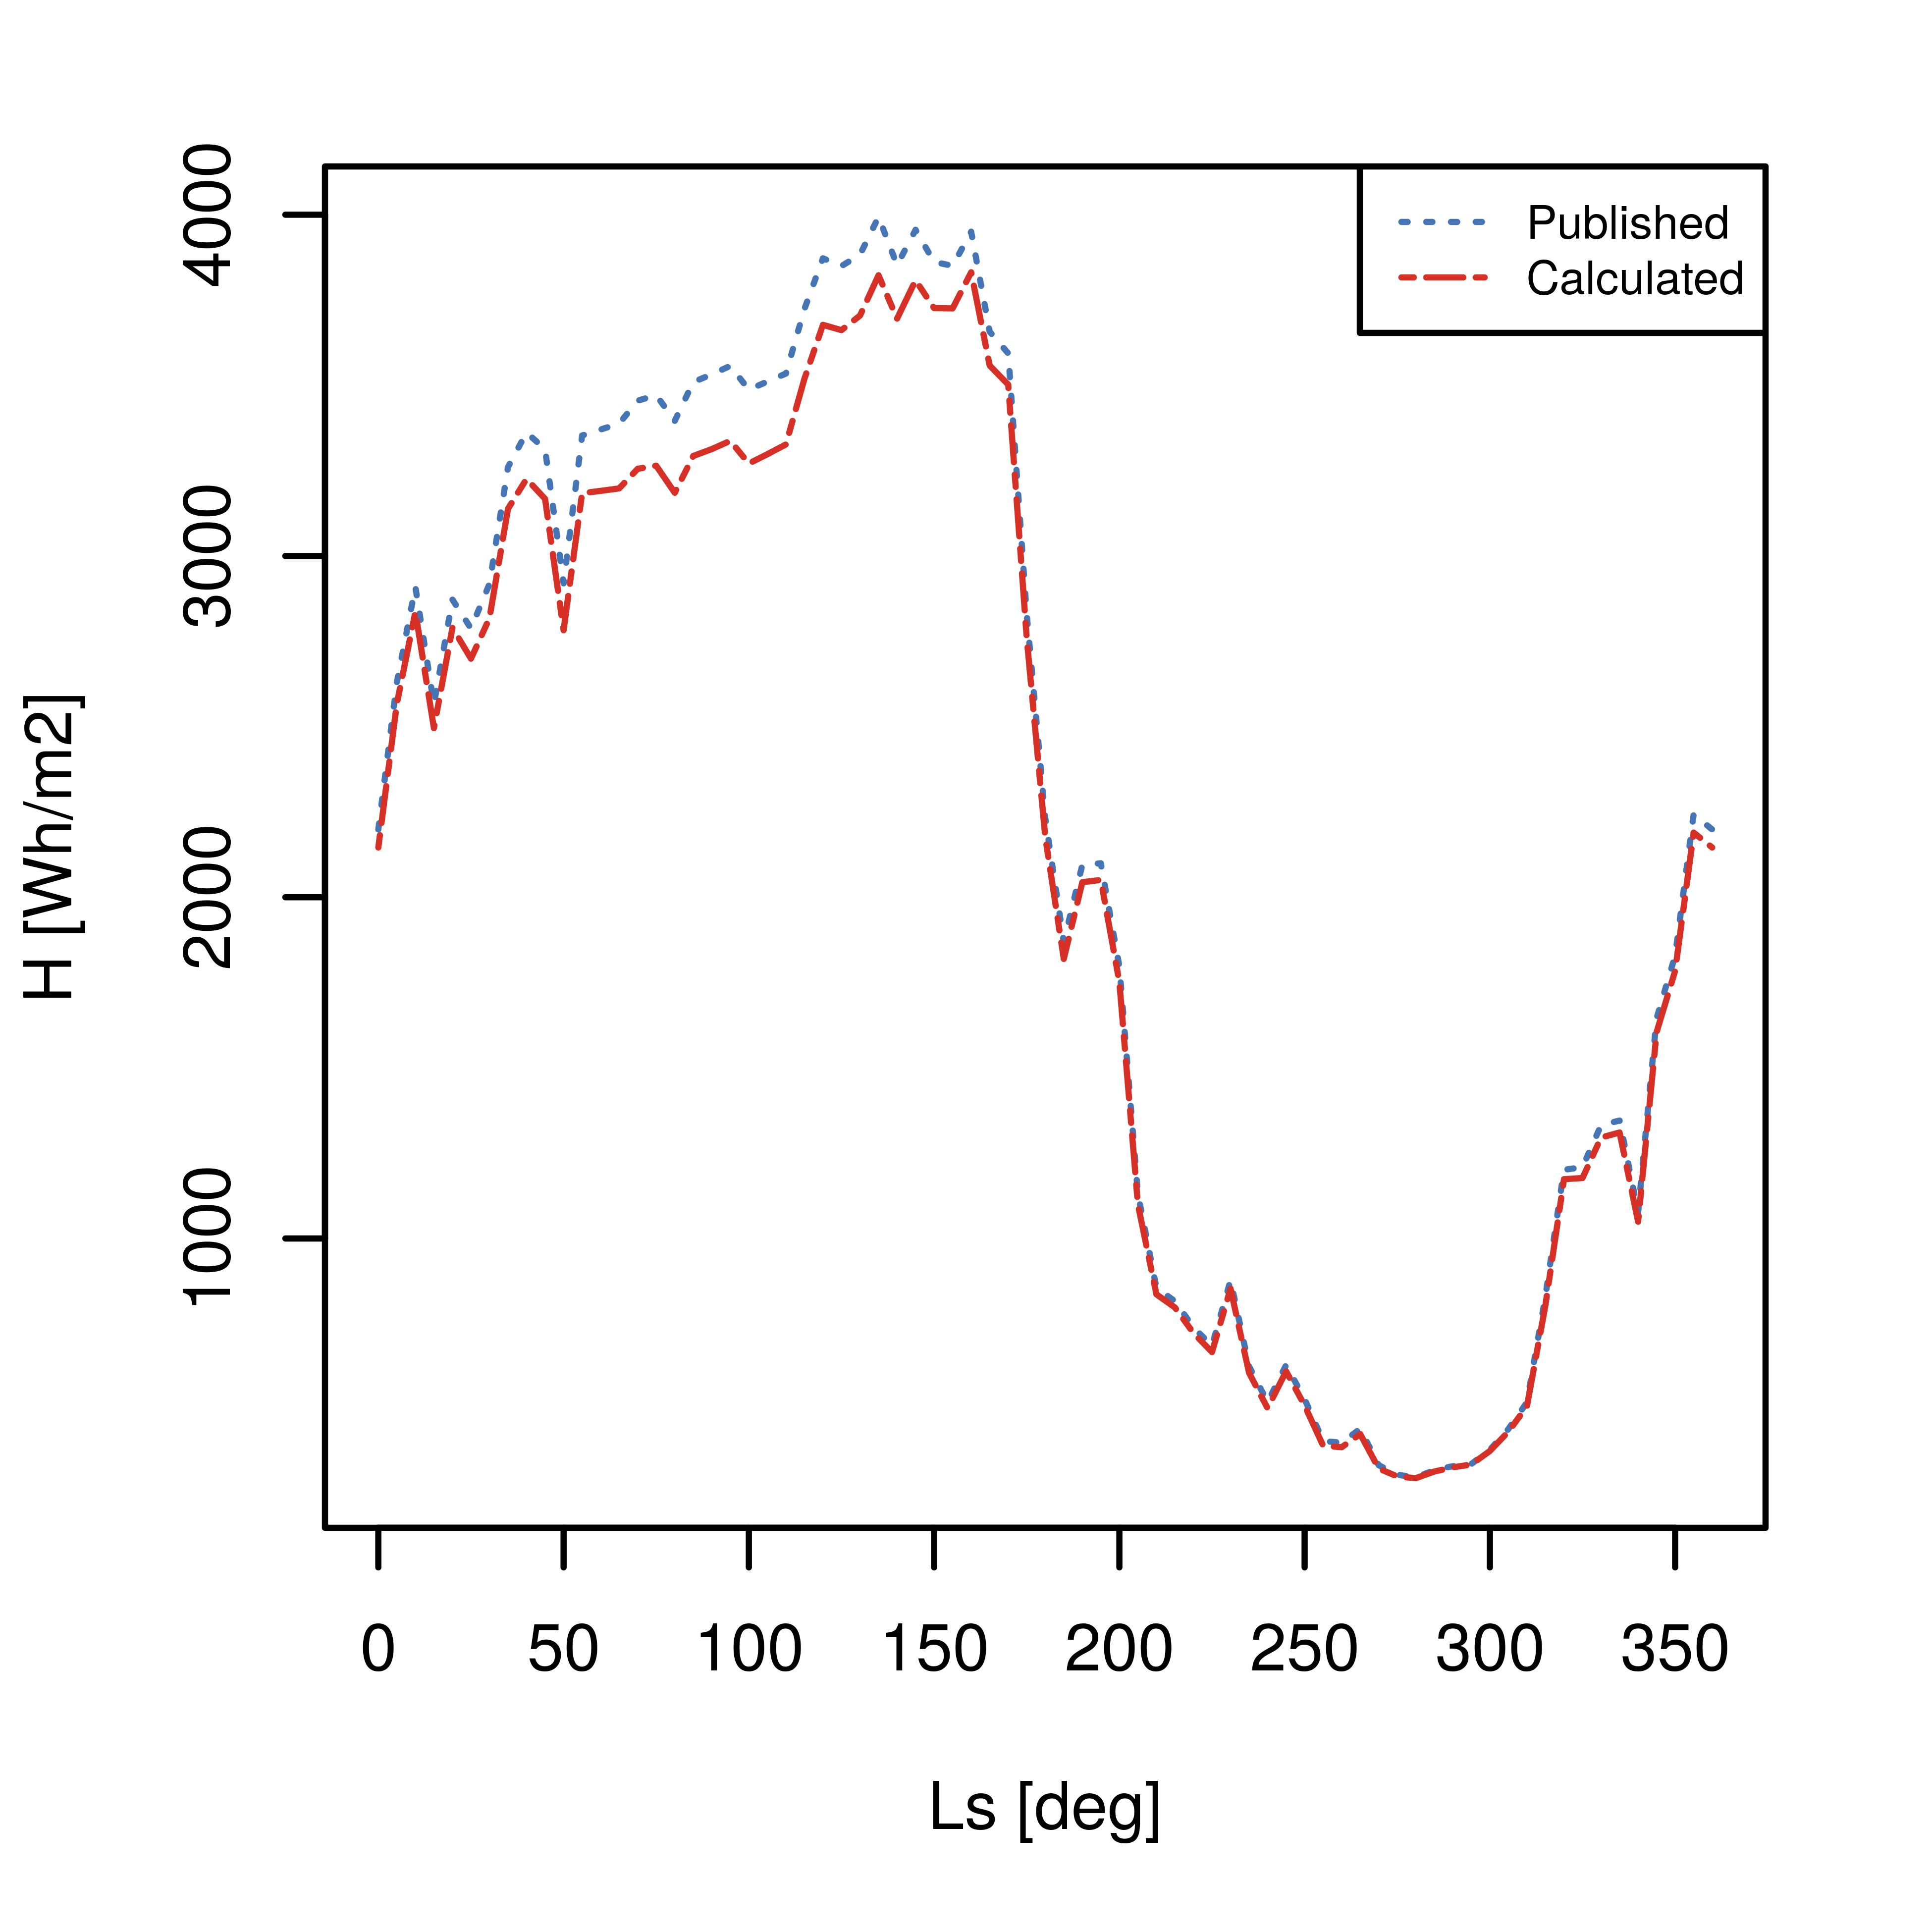
\includegraphics[height=\graphicsHeight]{sections/appendix/insolation-calculation-verification/plots/h-exp-calc-at-vl2-with-beta-477-deg.png}
            \subcaption{Daily variations}
            \label{fig:sub:comparative-global-insolation-at-vl2-beta-equals-phi-daily-variations}
    \end{subfigure}\hfill
    \begin{subfigure}[t]{\subfigureWidth}
        \centering
            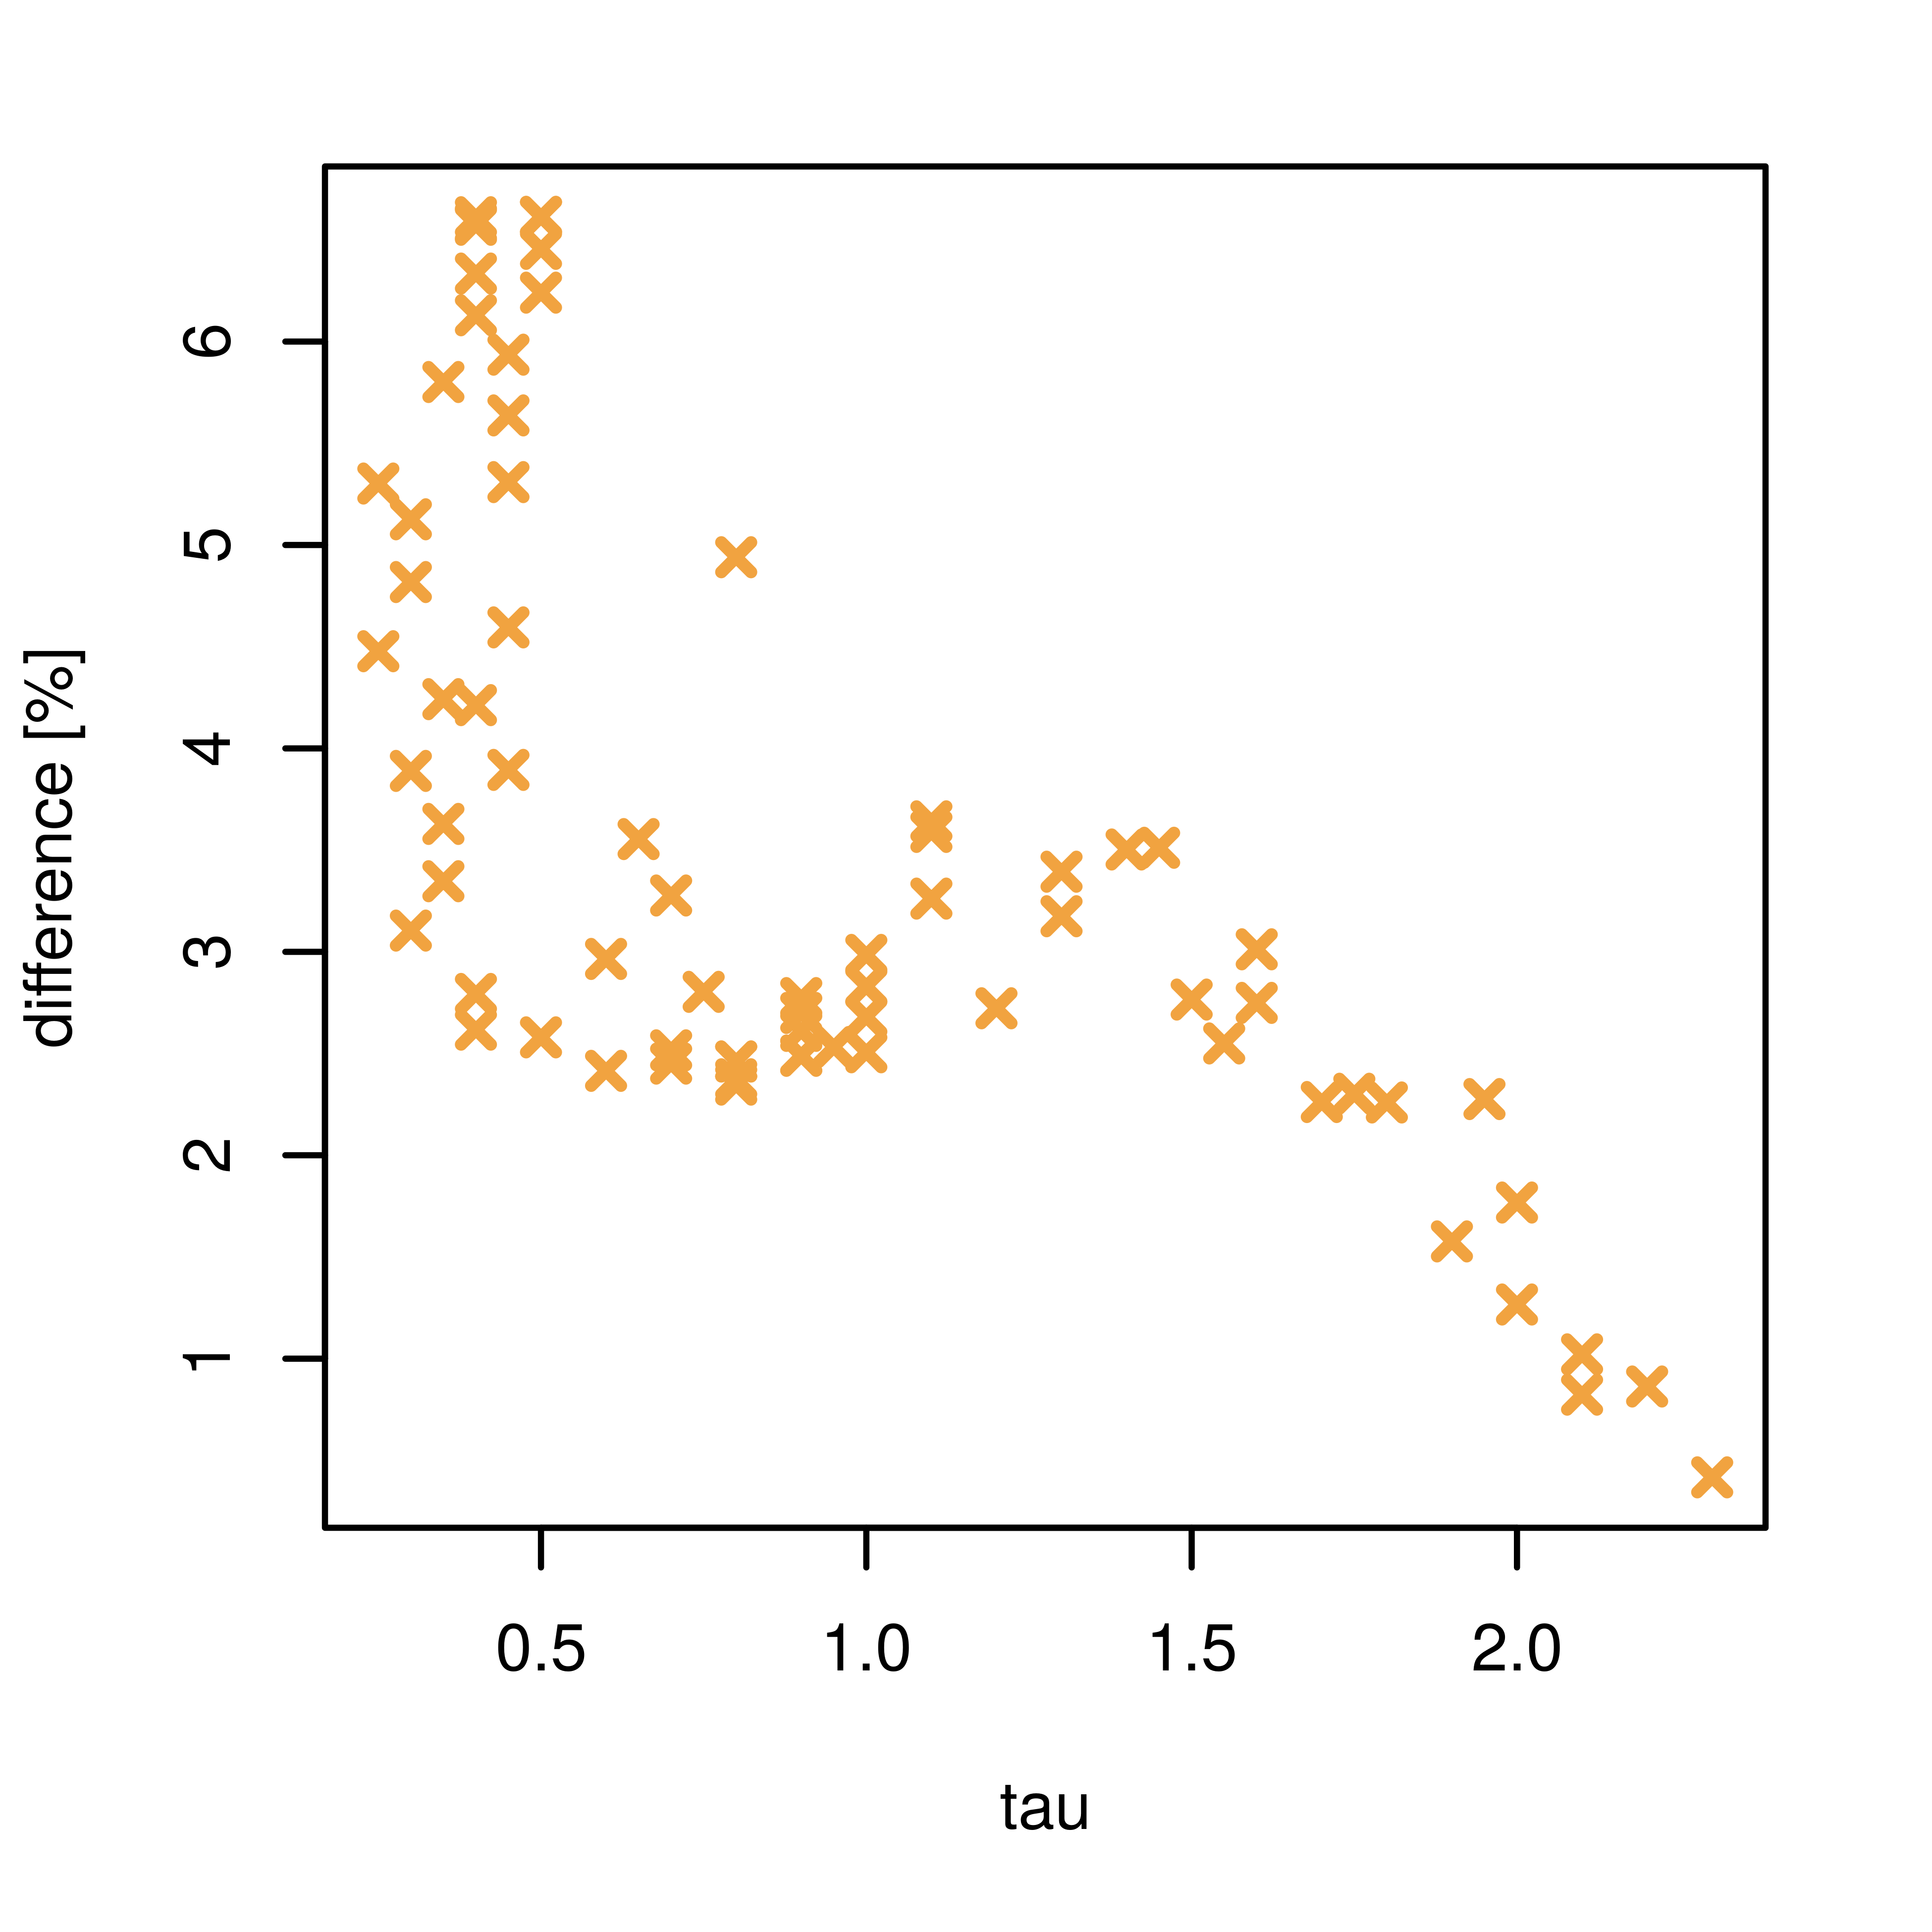
\includegraphics[height=\graphicsHeight]{sections/appendix/insolation-calculation-verification/plots/h-diff-bet-exp-calc-at-vl2-with-beta-477-deg.png}
            \subcaption{Differences as a function of optical depth}
            \label{fig:sub:comparative-global-insolation-at-vl2-beta-equals-phi-percentage-differences}
    \end{subfigure}\\[0.8ex]
    \caption[Daily global insolations at Viking Lander 2 on an inclined surface with $\beta=\SI{47.7}{\degree}$]
    {Daily global insolations at \ac{VL2} on an inclined surface with $\beta=\SI{47.7}{\degree}$.}
    \label{fig:plot:comparative-global-insolation-at-vl2-beta-equals-phi}
\vspace{-2ex}
\end{figure}

\section{Inclined Surface with Optimal Beta Angle}
\subsection{At Viking Lander 1 (VL1)}
\refFig{fig:sub:comparative-global-insolation-at-vl1-beta-optimal-daily-variations} shows that calculated values are consistently lower than those published in \citemarsenv{Appelbaum1993}. Both daily variations closely follow the same pattern. \refFig{fig:sub:comparative-global-insolation-at-vl1-beta-optimal-percentage-differences} reveals that the differences between calculated and published values range between \SI{2}{\percent} and \SI{2.8}{\percent}. Differences larger than \SI{2.5}{\percent} are more frequent for large $\tau$ values starting from 1.9.

\begin{figure}[h]
\captionsetup[subfigure]{justification=centering}
\vspace{-2ex}
\centering
    %% setup sizes
    \setlength{\subfigureWidth}{0.50\textwidth}
    \setlength{\graphicsHeight}{60mm}
    %% kill hyper-link highlighting
    \hypersetup{hidelinks=true}%
    %% the figures
    \begin{subfigure}[t]{\subfigureWidth}
        \centering
            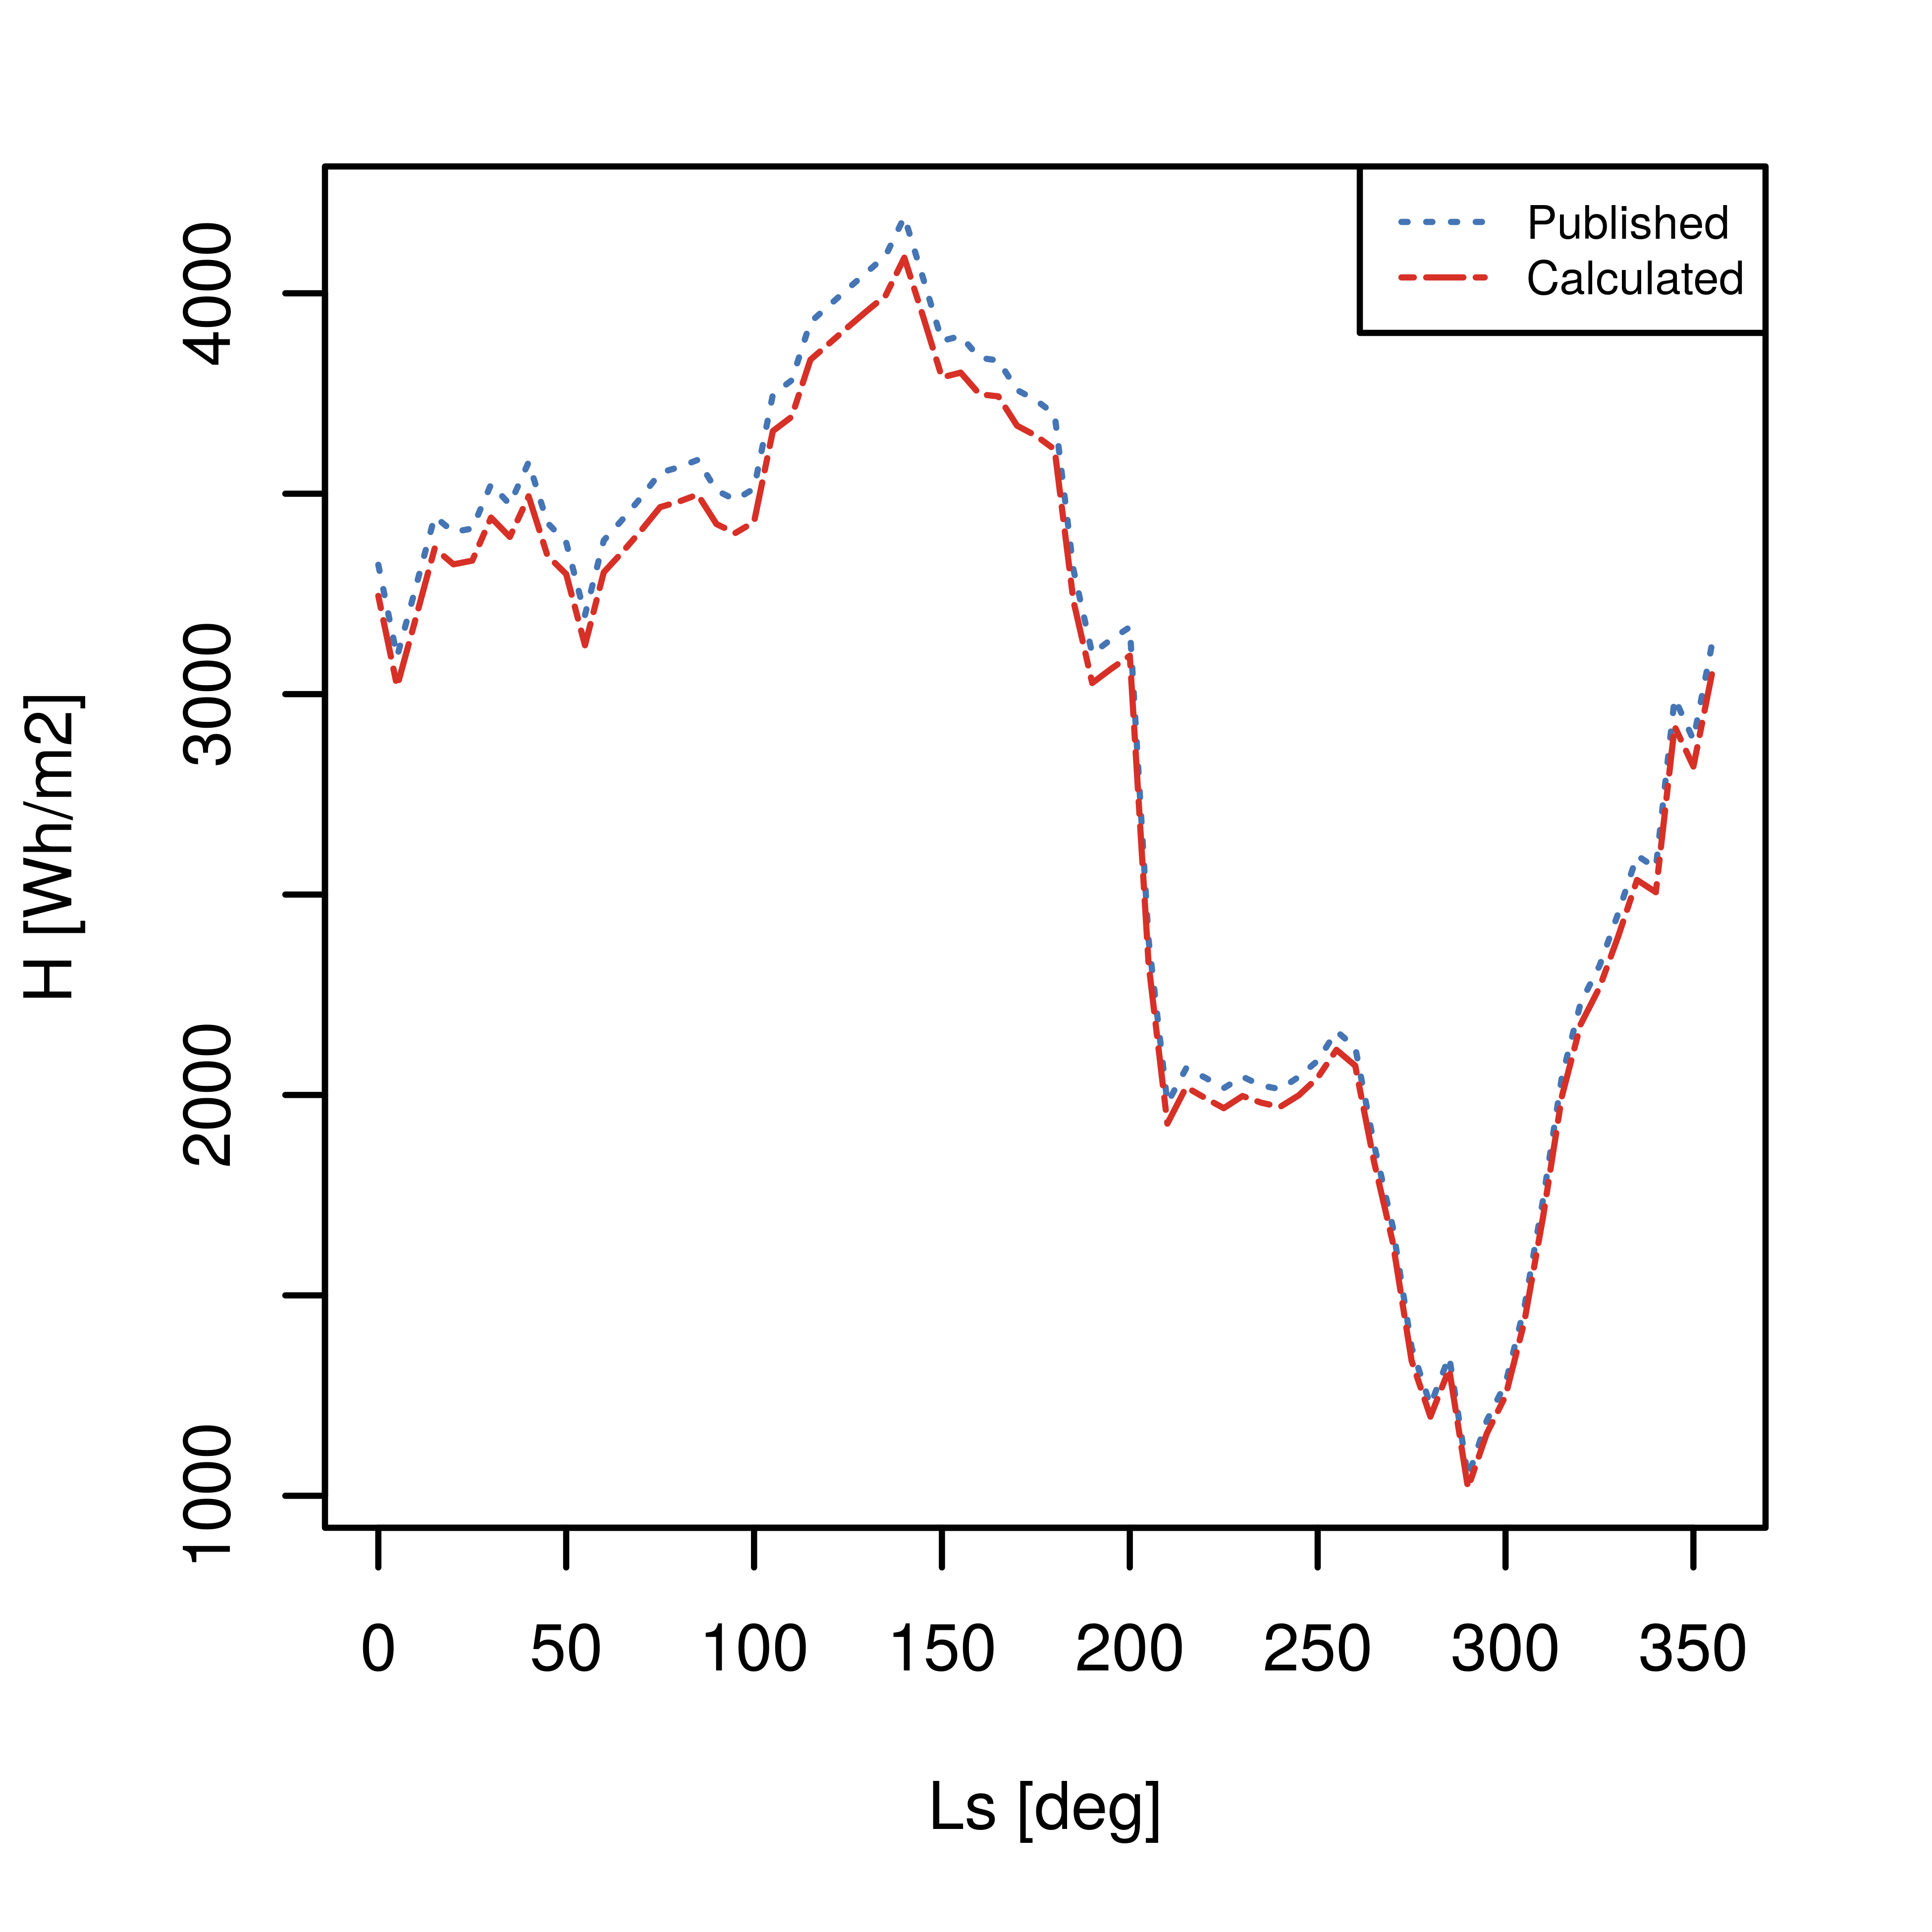
\includegraphics[height=\graphicsHeight]{sections/appendix/insolation-calculation-verification/plots/h-exp-calc-at-vl1-with-beta-65-deg.png}
            \subcaption{Daily variations}
            \label{fig:sub:comparative-global-insolation-at-vl1-beta-optimal-daily-variations}
    \end{subfigure}\hfill
    \begin{subfigure}[t]{\subfigureWidth}
        \centering
            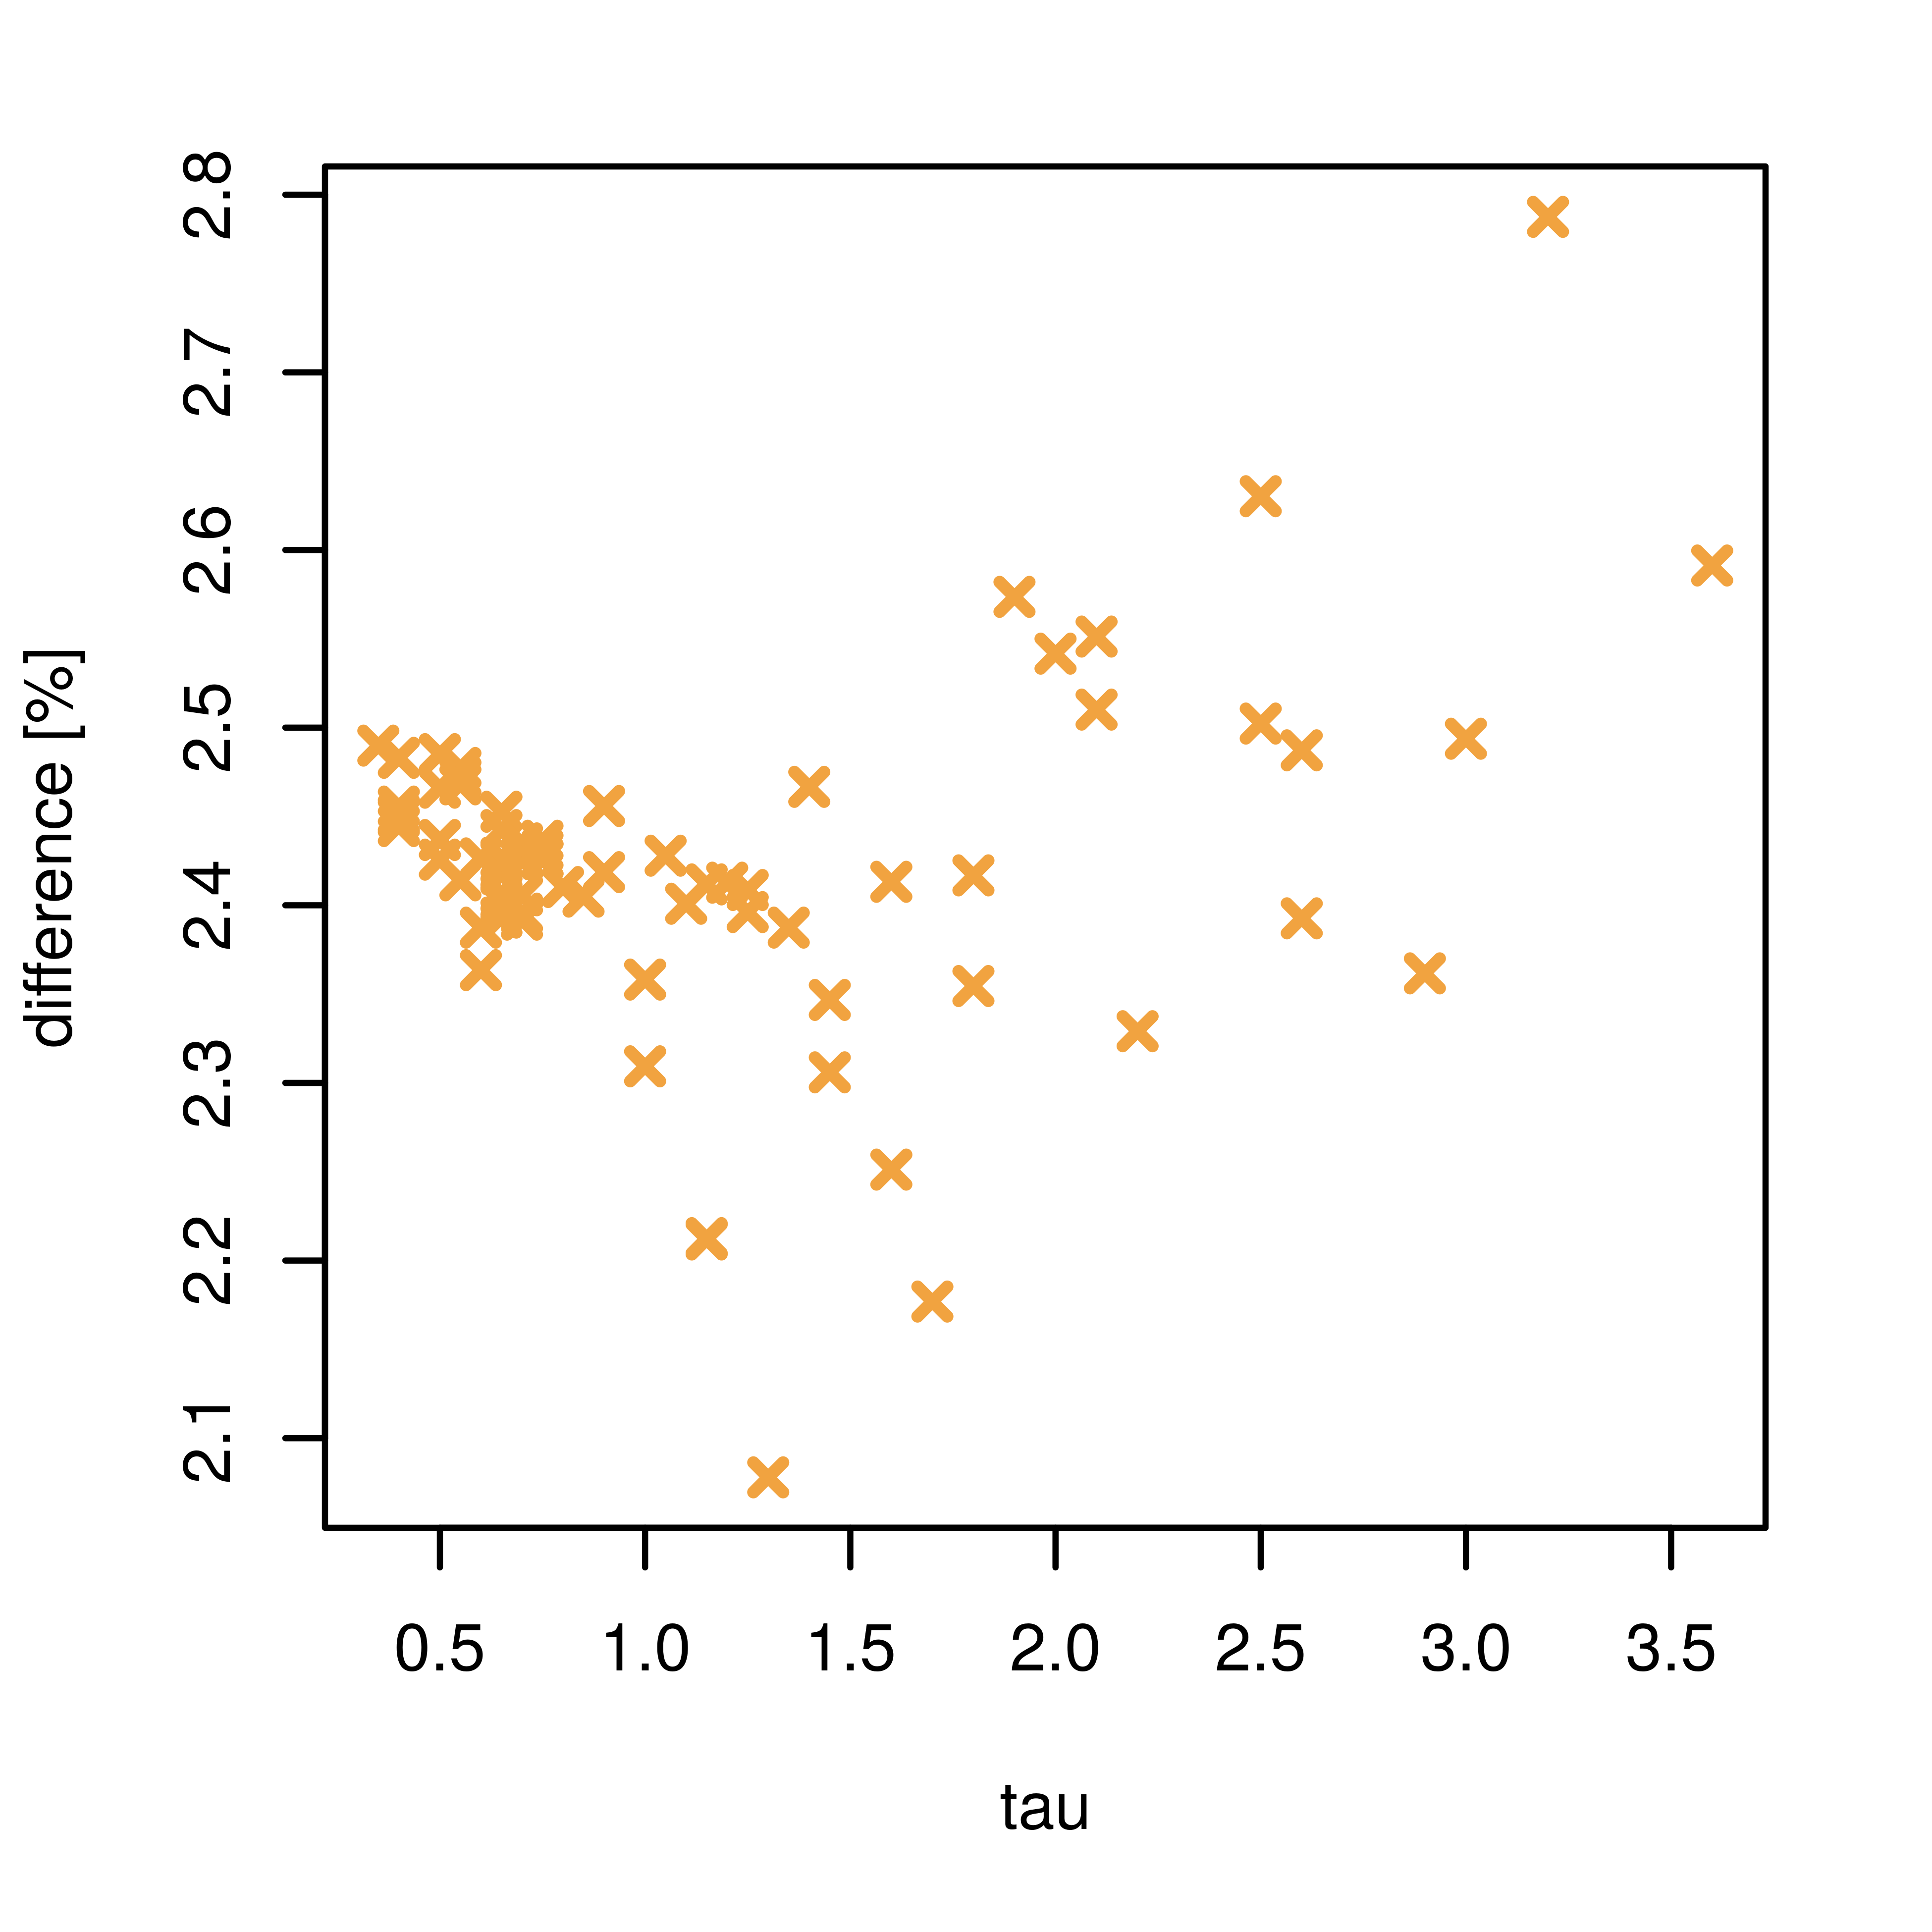
\includegraphics[height=\graphicsHeight]{sections/appendix/insolation-calculation-verification/plots/h-diff-bet-exp-calc-at-vl1-with-beta-65-deg.png}
            \subcaption{Differences as a function of optical depth}
            \label{fig:sub:comparative-global-insolation-at-vl1-beta-optimal-percentage-differences}
    \end{subfigure}\\[0.8ex]
    \caption[Daily global insolations at Viking Lander 1 on an inclined surface with $\beta=\SI{6.5}{\degree}$]
    {Daily global insolations at \ac{VL1} on an inclined surface with $\beta=\SI{6.5}{\degree}$.}
    \label{fig:plot:comparative-global-insolation-at-vl1-beta-optimal}
\vspace{-2ex}
\end{figure}

\subsection{At Viking Lander 2 (VL2)}
\refFig{fig:sub:comparative-global-insolation-at-vl2-beta-optimal-daily-variations} shows that calculated values are consistently lower than those published in \citemarsenv{Appelbaum1993}. Both daily variations closely follow the same patterns. \refFig{fig:sub:comparative-global-insolation-at-vl2-beta-optimal-percentage-differences} reveals that the differences between calculated and published values range between \SI{0.4}{\percent} and \SI{3.7}{\percent}. Differences larger than \SI{2.5}{\percent} are more frequent for small $\tau$ values, particularly below 1.6.

\begin{figure}[h]
\captionsetup[subfigure]{justification=centering}
%\vspace{-2ex}
\centering
    %% setup sizes
    \setlength{\subfigureWidth}{0.50\textwidth}
    \setlength{\graphicsHeight}{60mm}
    %% kill hyper-link highlighting
    \hypersetup{hidelinks=true}%
    %% the figures
    \begin{subfigure}[t]{\subfigureWidth}
        \centering
            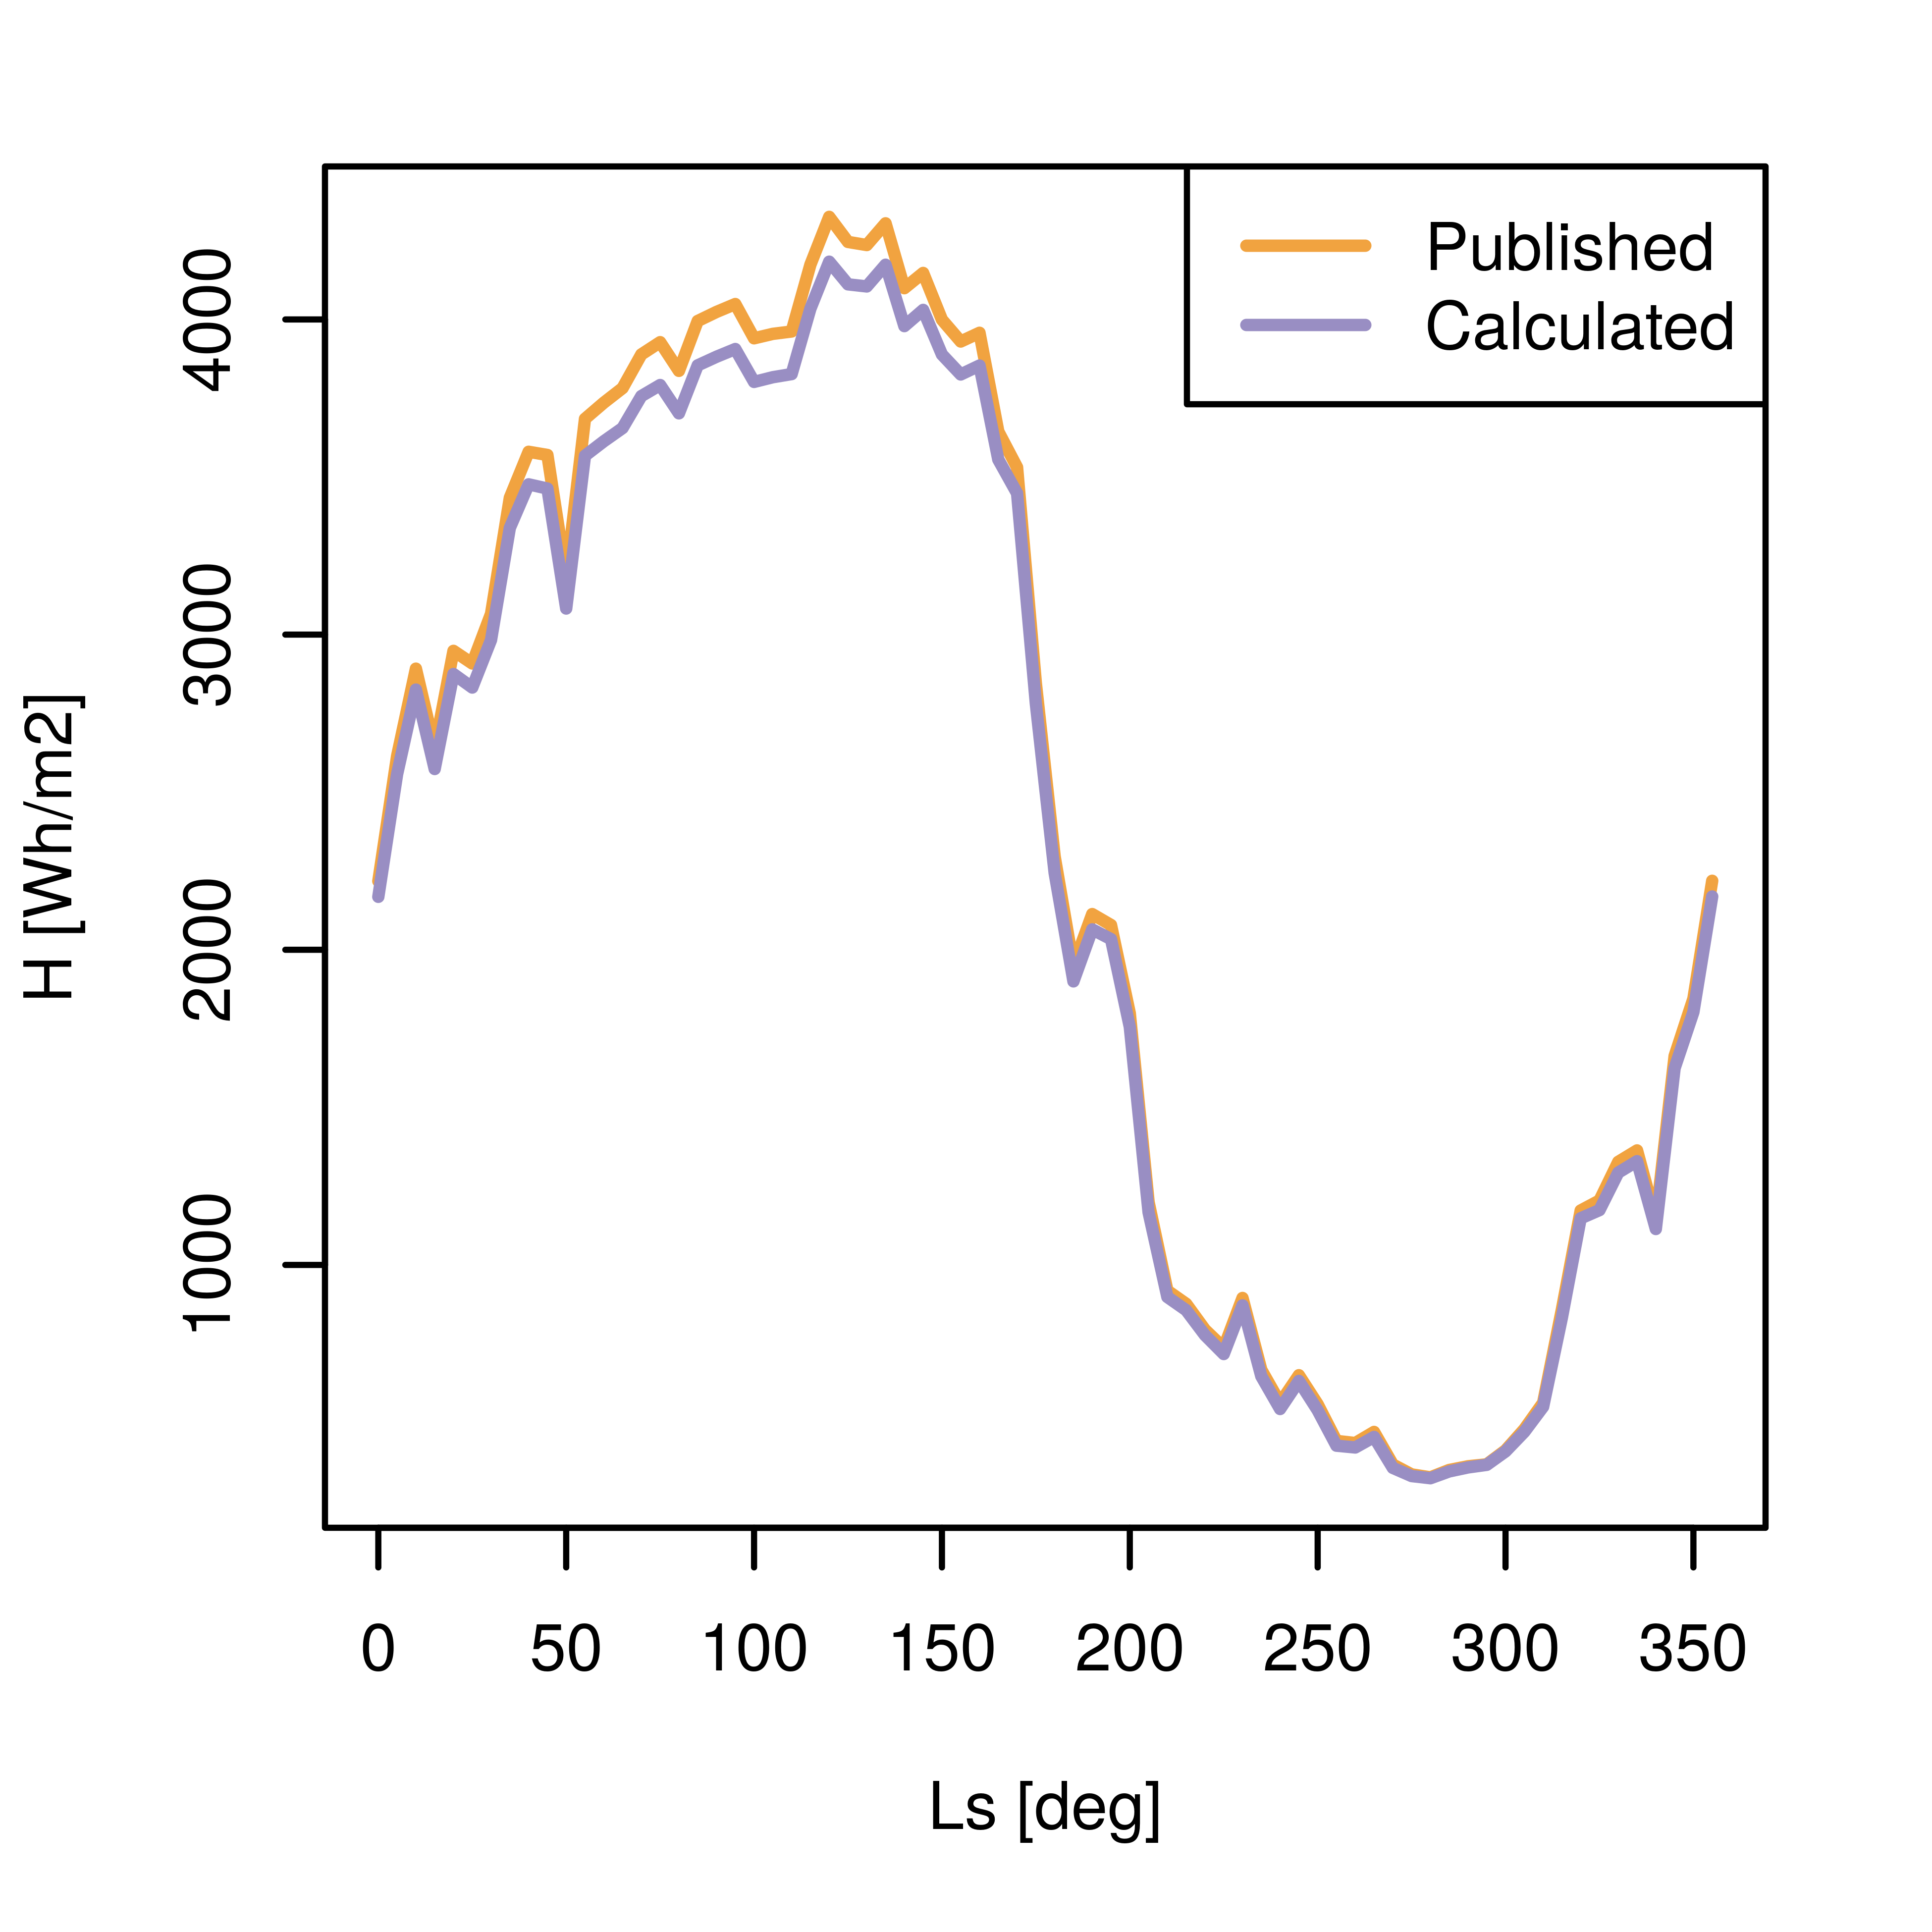
\includegraphics[height=\graphicsHeight]{sections/appendix/insolation-calculation-verification/plots/h-exp-calc-at-vl2-with-beta-22-deg.png}
            \subcaption{Daily variations}
            \label{fig:sub:comparative-global-insolation-at-vl2-beta-optimal-daily-variations}
    \end{subfigure}\hfill
    \begin{subfigure}[t]{\subfigureWidth}
        \centering
            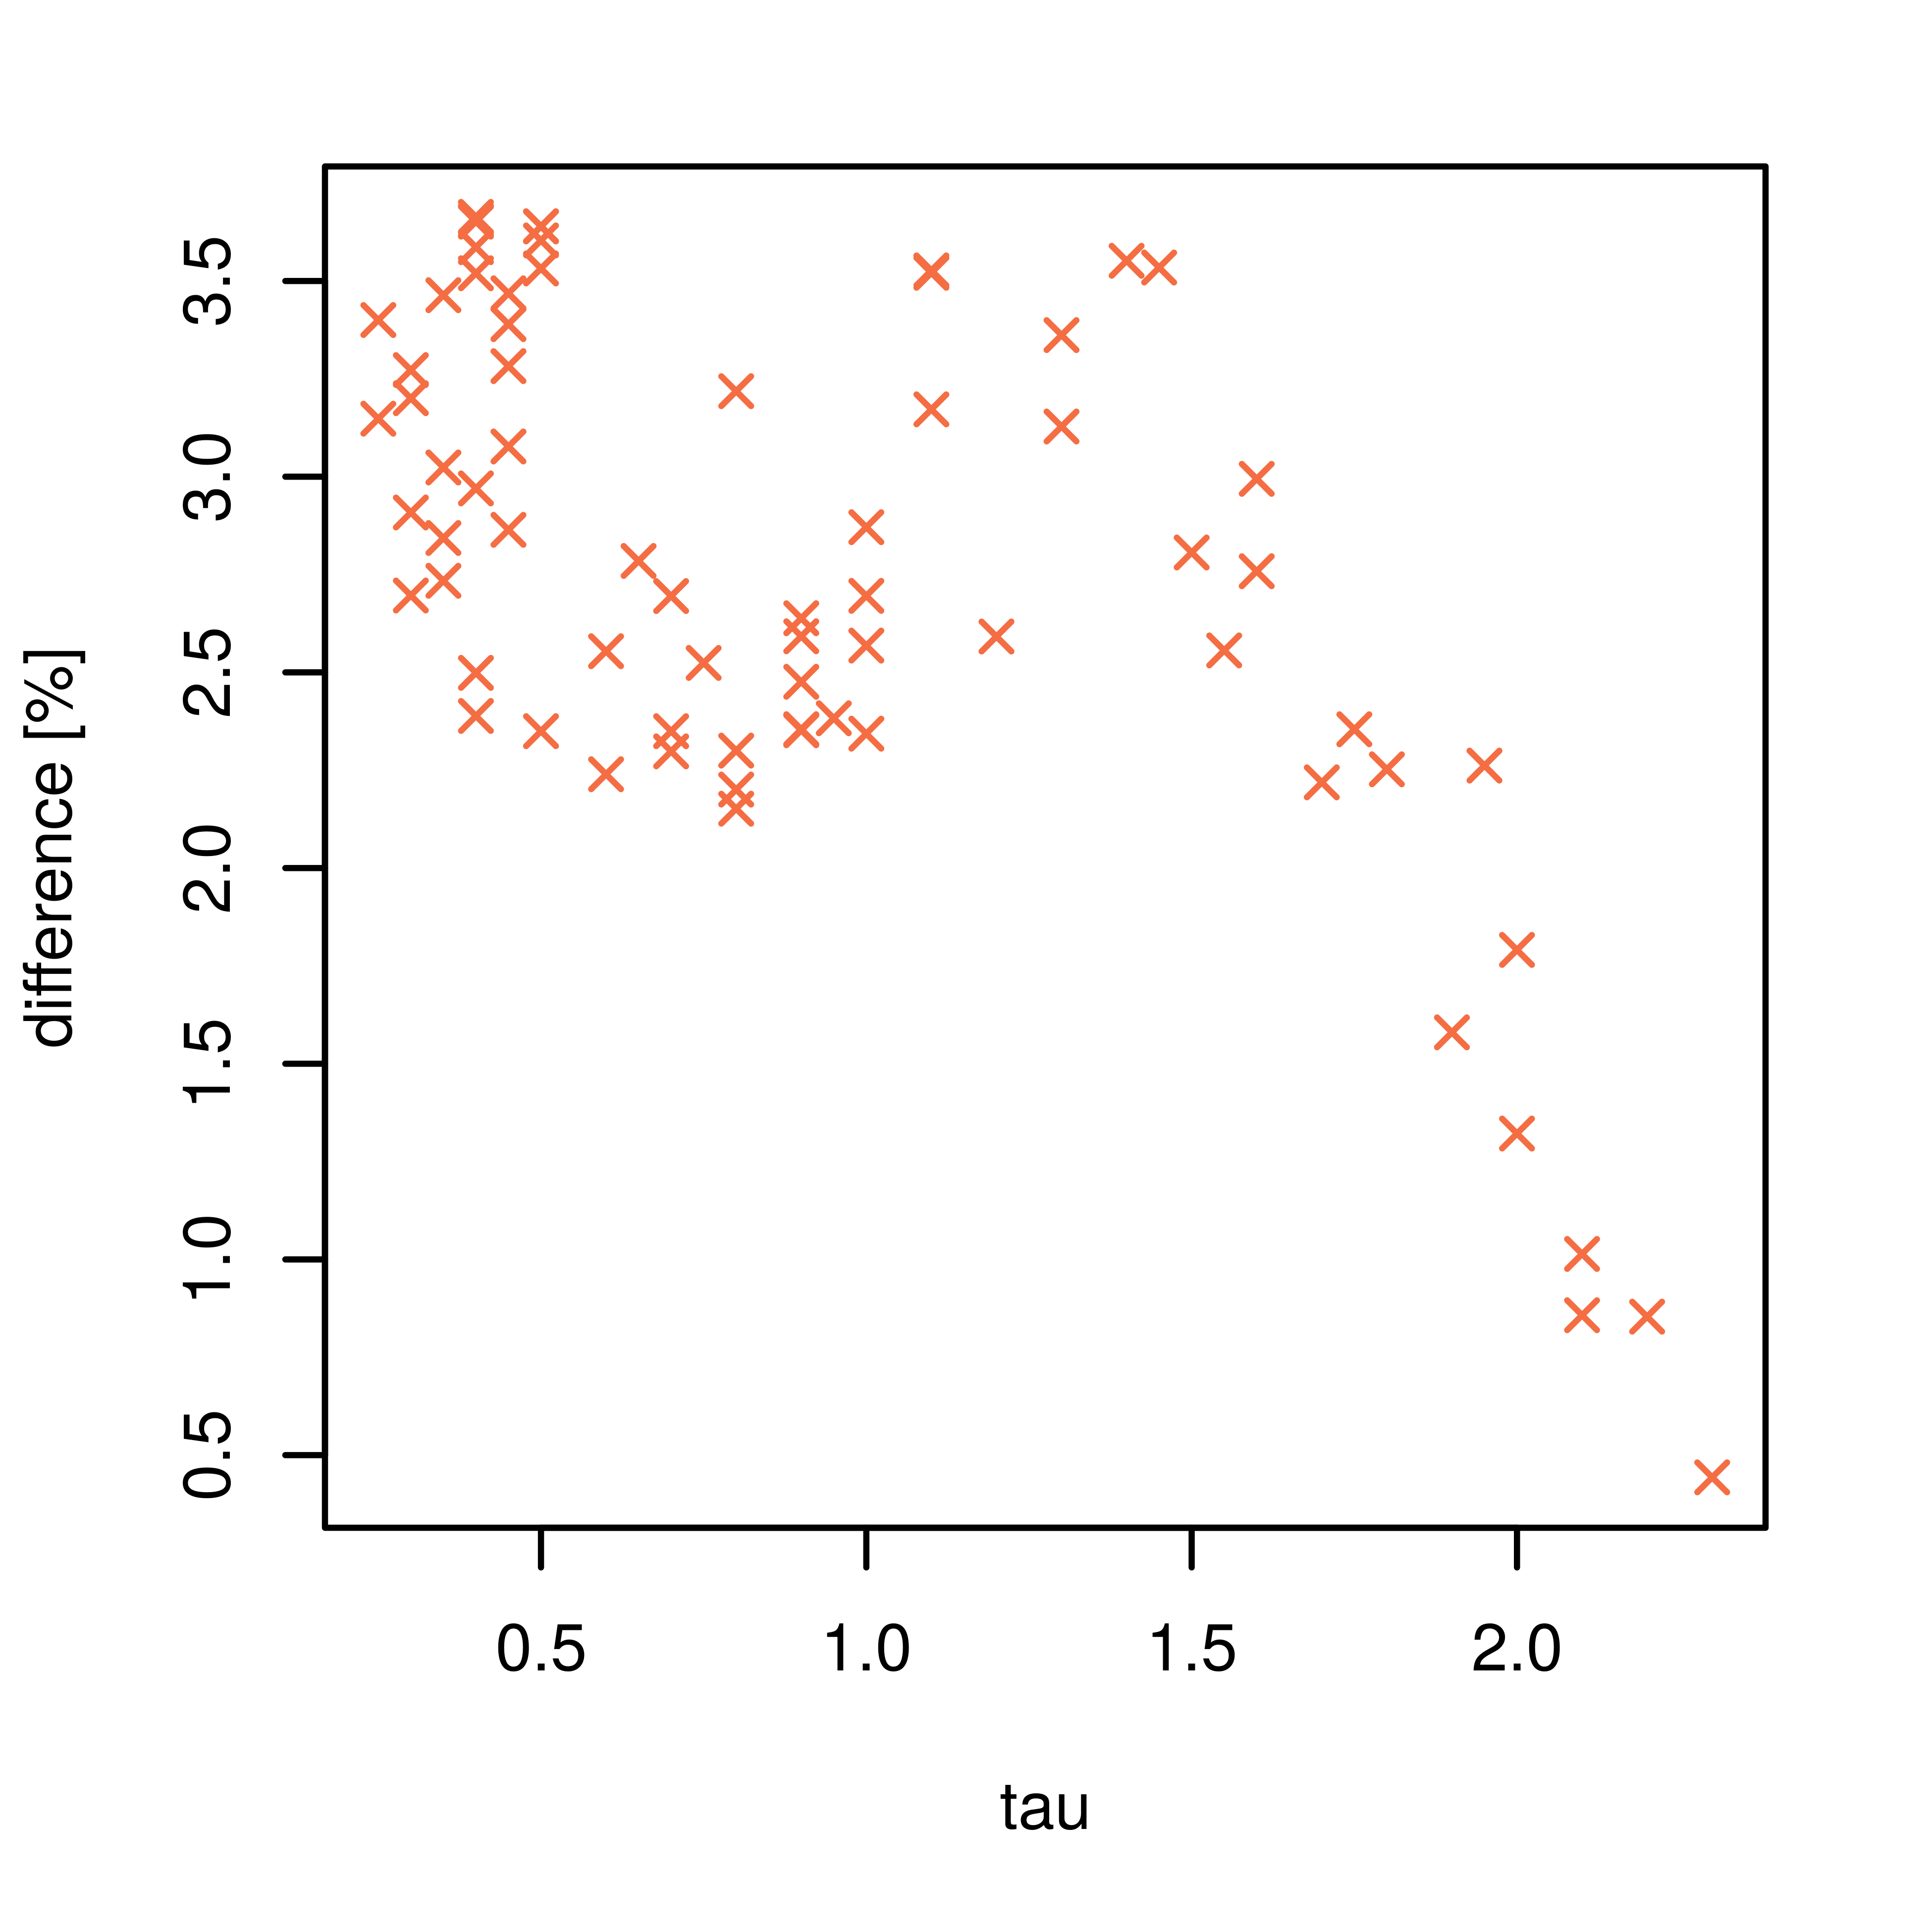
\includegraphics[height=\graphicsHeight]{sections/appendix/insolation-calculation-verification/plots/h-diff-bet-exp-calc-at-vl2-with-beta-22-deg.png}
            \subcaption{Differences as a function of optical depth}
            \label{fig:sub:comparative-global-insolation-at-vl2-beta-optimal-percentage-differences}
    \end{subfigure}\\[0.8ex]
    \caption[Daily global insolations at Viking Lander 2 on an inclined surface with $\beta=\SI{22}{\degree}$]
    {Daily global insolations at \ac{VL2} on an inclined surface with $\beta=\SI{22}{\degree}$.}
    \label{fig:plot:comparative-global-insolation-at-vl2-beta-optimal}
\vspace{-2ex}
\end{figure}

\section{Conclusion}
It is not fully understood why differences exist between published and calculated global insolation values considering that, to the best of the author's knowledge, the same input parameters is used in both cases. Not presented in this chapter are differences for the beam, diffuse, and albedo components that compose the global insolation. These do not suggest that a single component is the source of the issue. Analyzing the differences as a function of $\tau$ hints that the issue is closely related to $\tau$ value inputs. Possible explanations could be:
\begin{itemize}
    \item The normalized net flux function lookup tables are used for insolations presented in \citemarsenv{Appelbaum1990} and \citemarsenv{Appelbaum1993} rather than approxmiated via the polynomial expression.
    \item The albedo values is not approximated in the same manner for insolations presented in \citemarsenv{Appelbaum1993}.
    \item The analytical precision differs between the computational medium used to obtain the published insolations versus the calculations obtained with R.
\end{itemize}

Regardless of the observed differences, the outputs given by the R package is still used for the analysis in this thesis based on the following justifications:
\begin{itemize}
  \item The calculated global insolation values are lesser than those published. This introduces a conservative element from which mission analysis benefits in terms of mitigating against the risk of over-predicting power budgets and energy predictions.
  \item The largest differences are for smaller values of $\tau$. Mission analysis focuswa on larger $\tau$ values as they present the worst-case energy generation outcome with respect to the Martian dust environment.
  \item The differences between calculated and published values are small in terms of the resulting insolation relative to the total daily insolation.
  \item The calculated and published values closely follow the same daily variation pattern.
\end{itemize}
